\documentclass[a4wide]{report}

\usepackage{amsmath}
\usepackage[a4paper, total={7in, 10.2in}]{geometry}
\usepackage{graphicx}
\usepackage[portuguese]{babel}
\usepackage[utf8]{inputenc}


\begin{document}

\noindent
{\bf Rafael V. Cacilhas  - Relatório 04 (\today)}

\vspace{0.5cm}

\section*{Exercício 1}

\subsection*{a) }

Dada a relação de recorrência $x_{n+1} = 4rx_n(1-x_n)$ buscamos os pontos fixos e a estabilidade destes pontos. Pela definição de ponto fixo temos que:

\begin{equation*}
x^* = 4rx^*(1-x^*)
\end{equation*}

Claramente $x^* = 0$ é uma solução. Além desta, temos que:

\begin{equation*}
1 = 4r(1-x^*)
\end{equation*}

\begin{equation}
x^* = 1 - \frac{1}{4r}
\end{equation}

A estabilidade destes pontos fixos pode ser vista analisando o sinal de $f^{'}_{r}(r) = 4r - 8rx_n$. Para $x_n = 0$ temos que:


\begin{equation*}
|f^{'}_{r}(r)| < 1
\end{equation*}
\begin{equation*}
-1 <  4r  < 1
\end{equation*}

\begin{equation}
0 <  r  < 1/4
\end{equation}

Onde substituimos a solução $r > -1/4$ por $r > 0$, pois $r$ não pode ser negativo.

Para $x_n = 1 - \frac{1}{4r}$ temos:
\begin{equation*}
|f^{'}_{r}(r)| < 1
\end{equation*}
\begin{equation*}
-1 <  -4r + 2  < 1
\end{equation*}
\begin{equation}
\frac{1}{4} <  r  < \frac{3}{4}
\end{equation}


Assim sendo, vemos que para $r < 0.25$ temos que $x^* = 0$ é um ponto fixo estável e que para $0.25 < r < 0.75$ temos um ponto estável dependente de r, dado por  $x^* = 1 - \frac{1}{4r}$.

\subsection*{b)}

Para r = 0.24, temos que $x_{esperado}^{*} = 0$ e $x_{500} \approx 3.8\times10^{-11}$. As trajetórias, mostradas na Figura \ref{a1}, convergem para um mesmo valor próximo de zero, independente de $x_0$, como esperado pela análise feita anteriormente. O valor exato de $x_{500}$ pode ser visto na saída de dados do programa na tela.
\begin{figure}[!htb]
\centering
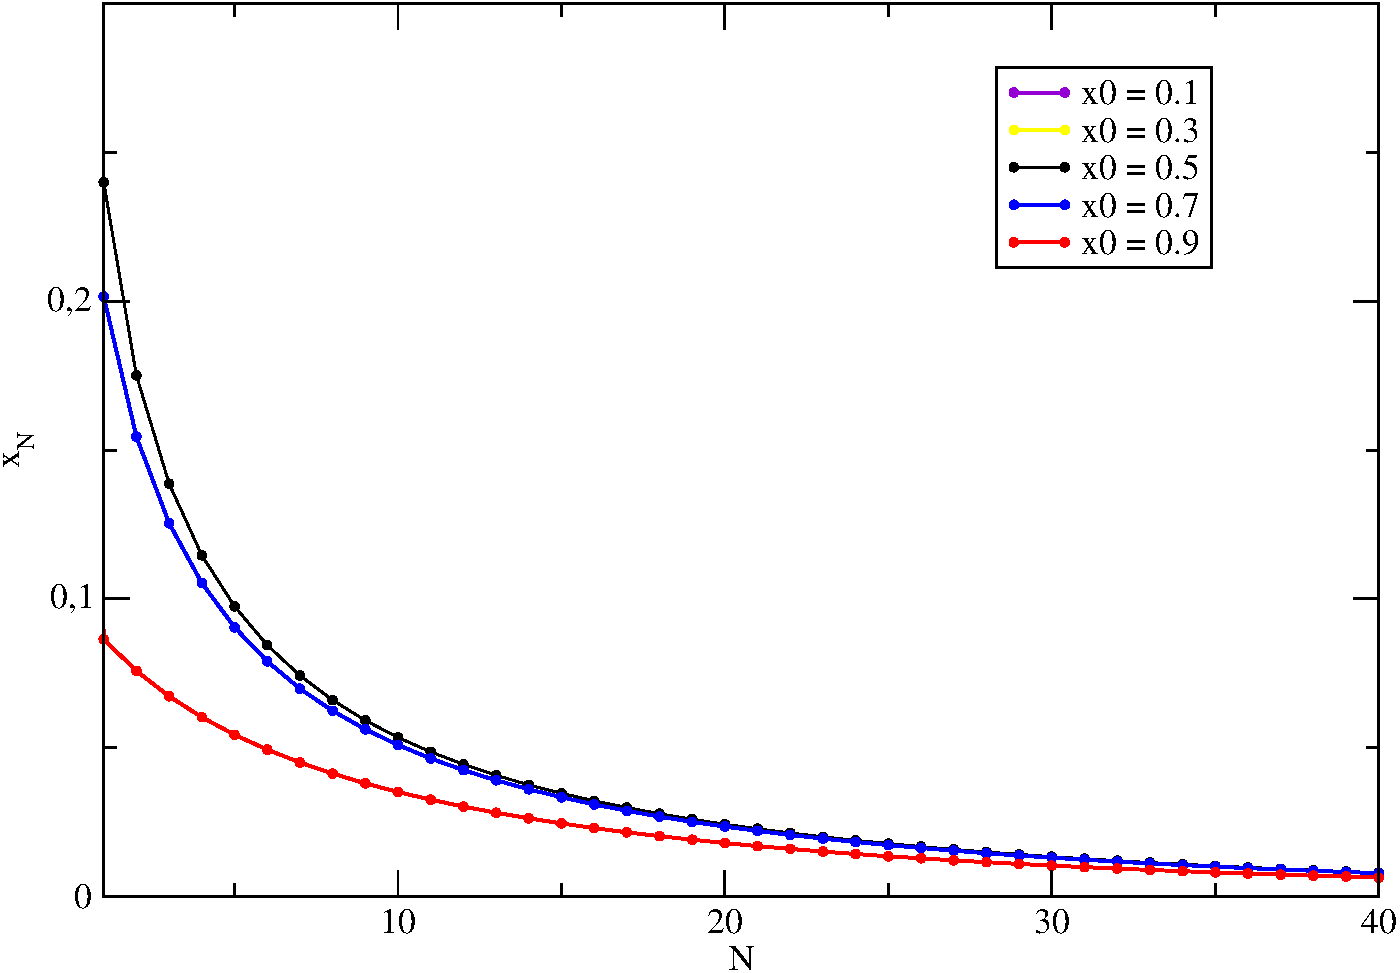
\includegraphics[width=0.447\textwidth]{todos.pdf}
\caption{Trajetórias para r = 0.24 para diferentes valores iniciais de x.}
\label{a1}
\end{figure}


Para r = 0.26, temos que $x_{esperado}^{*} \approx 3.8\times10^{-2}$ e $x_{500} \approx 3.8\times10^{-2}$, havendo divergência apenas na nona casa decimal. As trajetórias, mostradas na Figura \ref{a2}, convergem para um mesmo valor pouco abaixo de $5\times10^{-2}$, independente de $x_0$, como esperado pela análise feita anteriormente. Os valores exatos de $x_{esperado}^{*}$ e $x_{500}$ podem ser vistos na saída de dados do programa na tela.
\begin{figure}[!htb]
\centering
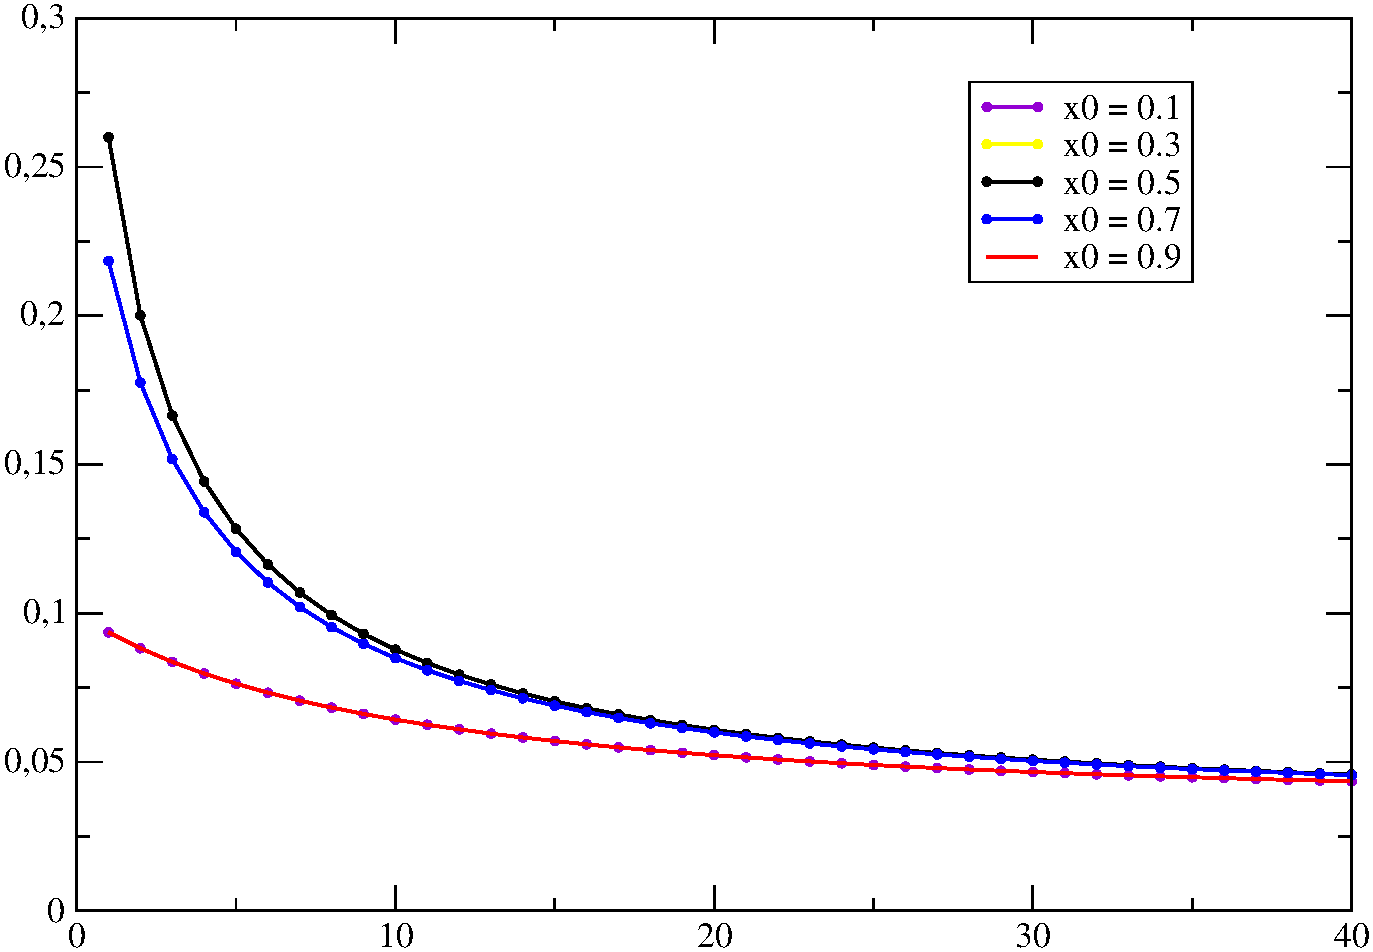
\includegraphics[width=0.447\textwidth]{todos26.pdf}
\caption{Trajetórias para r = 0.26 para diferentes valores iniciais de x. }
\label{a2}
\end{figure}

Assim, verificamos que os resultados obtidos estão de acordo com a análise de estabilidade feita anteriormente. Para $r < 0.25$ a trajetória se encaminha para perto de zero (que é o ponto fixo) independente do valor inicial (já que o ponto fixo é estável). Para $r > 0.25$ a trajetória converge para um valor próximo de $3.8\times10^{-2}$ (que é o ponto fixo) independente do valor inicial de x (já que é um ponto fixo estável).




\subsection*{ c) }

Foi mostrado anteriormente que para r entre 0.25 e 0.75 temos um ponto fixo estável dado por $x^* = 1 - \frac{1}{4r}$. Utilizando a variável auxiliar $r' = 1/r$ temos que $x^* = 1 - \frac{1}{4}r'$ para $1.33 < r' < 4$, ou seja, uma relação linear em r'. Os pontos fixos encontrados para diferentes r' estão no gráfico da Figura \ref{c)}. Como esperado, há uma relação linear entre x* e $\frac{1}{r}$ neste intervalo de r.

\begin{figure}[!htb]
\centering
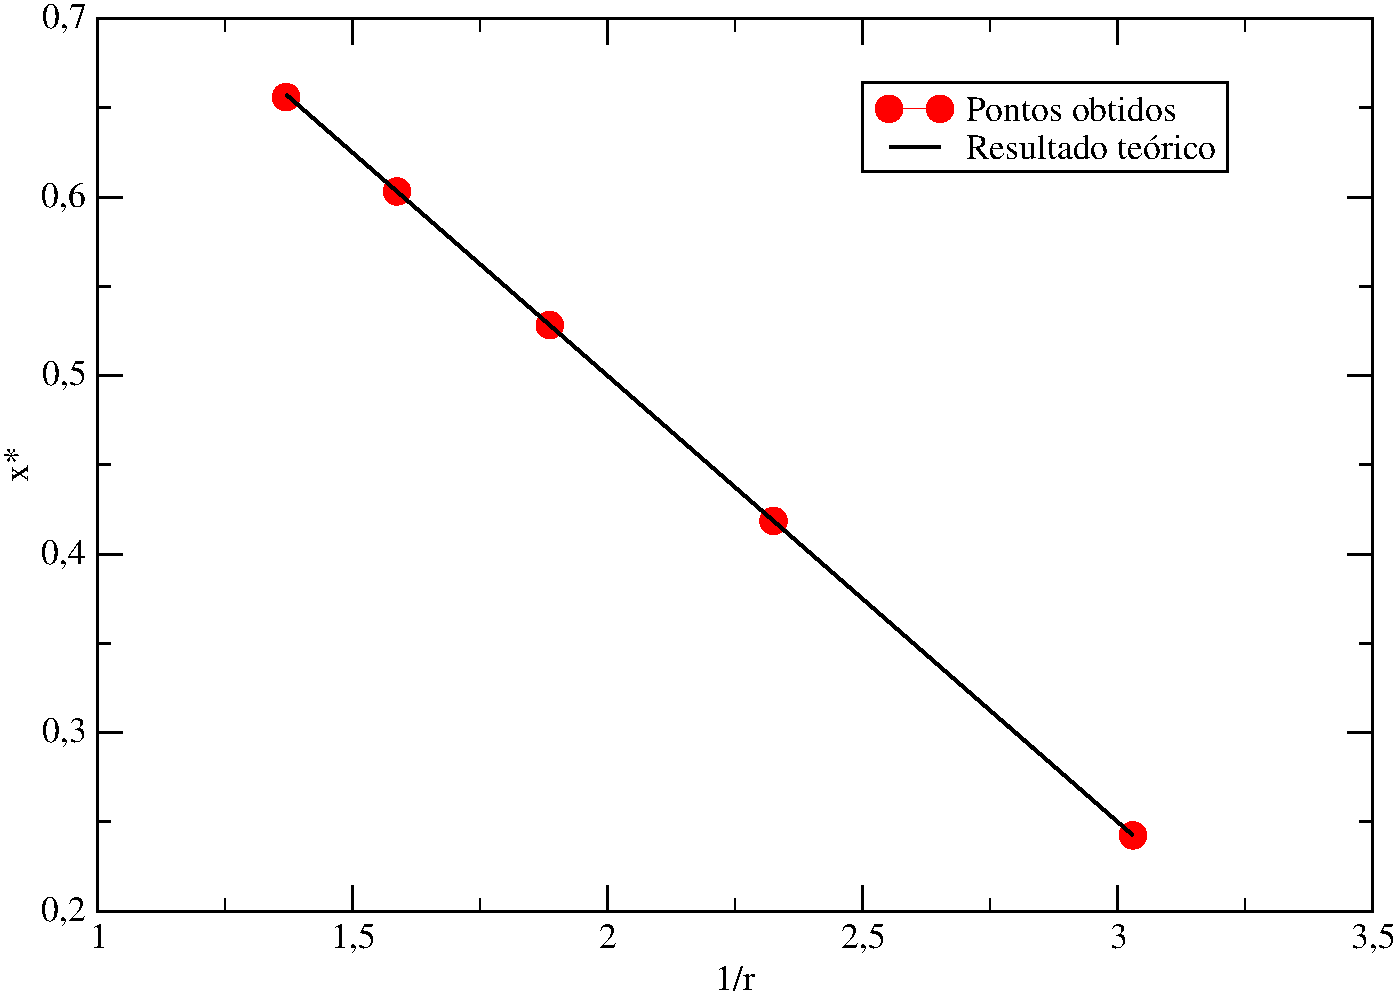
\includegraphics[width=0.447\textwidth]{1r.pdf}
\caption{x* em função de 1/r.}
\label{c)}
\end{figure}



\subsection*{ d) }

Para cada valor de $(x_0,r)$ foi feito um gráfico da trajetória $x_n$. Com o gráfico original não é possível ver o valor exato do período, então foi feito um zoom em uma região arbitrária de modo a se verificar qual é este valor. Um exemplo disso está na Figura \ref{085}, onde vemos que o perído é $p = 2$. Para os outros valores de $(x_0,r)$ foi omitido o gráfico com zoom, visto que basta utilizar a ferramenta de zoom do programa usado pra fazer o gráfico.

\begin{figure}[!htb]
\centering
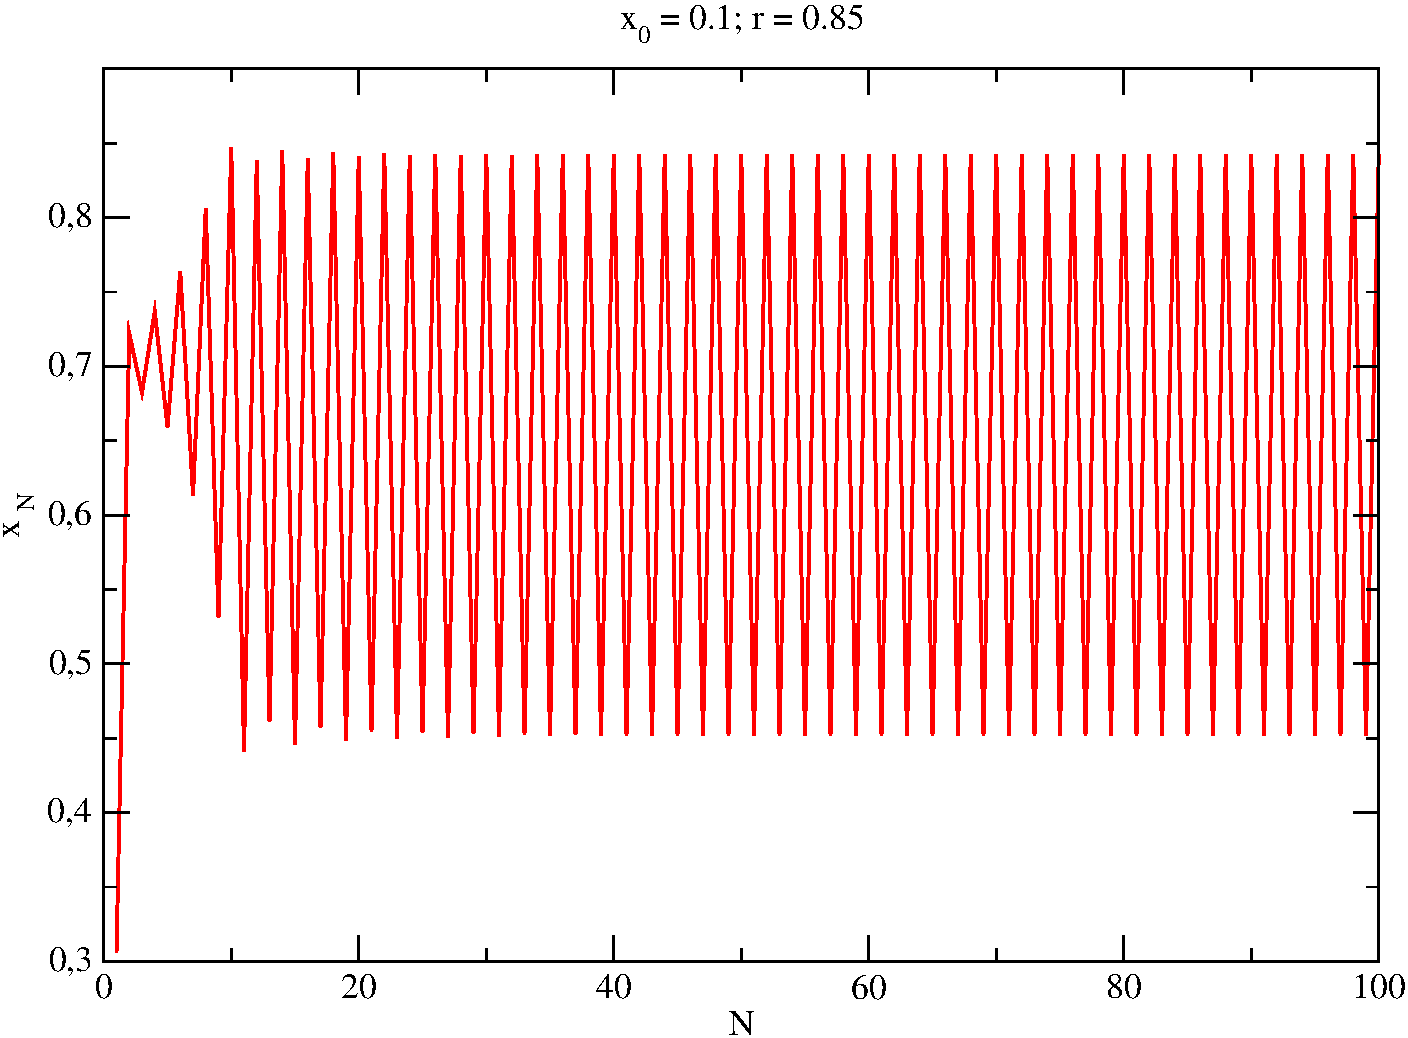
\includegraphics[width=0.447\textwidth]{085.pdf}
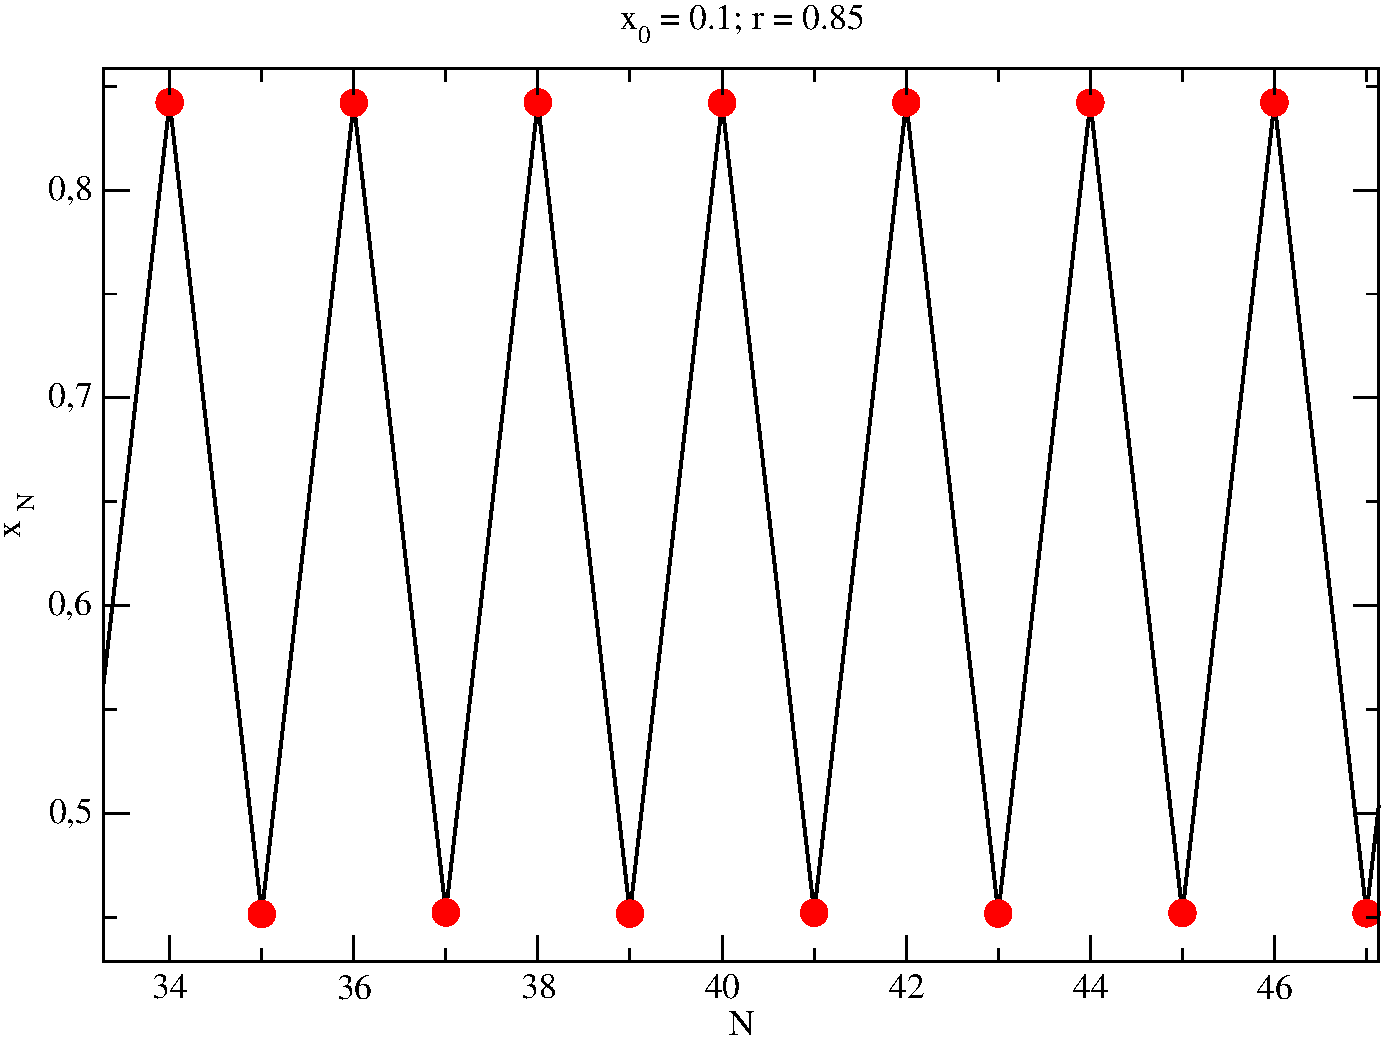
\includegraphics[width=0.447\textwidth]{085zoom.pdf}
\caption{Resultado para $x_0 = 0.1$ e $r = 0.85$ (esquerda) e um zoom em uma região arbitrária para evidenciar o período (direita). }
\label{085}
\end{figure}

O perído obtido para $x_0 = 0.1$ para todos os valores de r foram:
$\begin{cases} 
p(0.85) = 2 \\ 
p(0.87) = 4 \\
p(0.89) = 8 \\
p(0.96) = 3
\end{cases} $

Para $x_0 = 0.9$ temos que os valores do período devem ser os mesmos, pois os valores de $x_n$ são os mesmos para $x_0 = 0.1$ e $x_0 = 0.9$ para $n > 0$. O programa apresentou os mesmos resultados, como esperado; eles serão omitidos aqui visto que são idênticos aos apresentados, mas podem ser conferidos na pasta correspondente.


\begin{figure}[!htb]
\centering
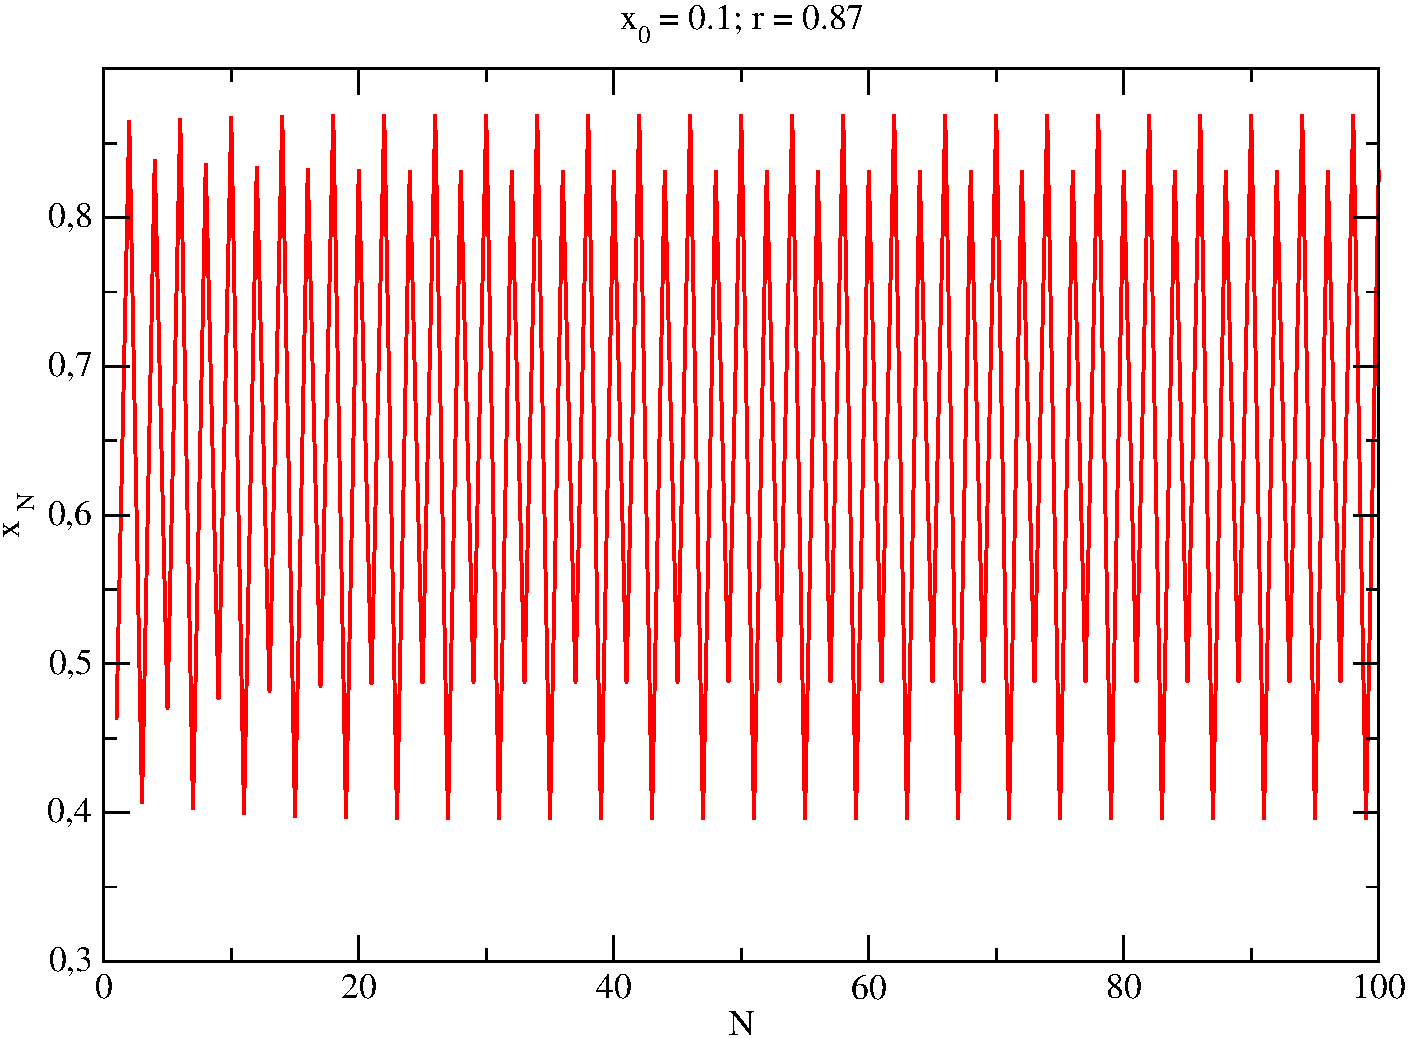
\includegraphics[width=0.447\textwidth]{087.pdf}
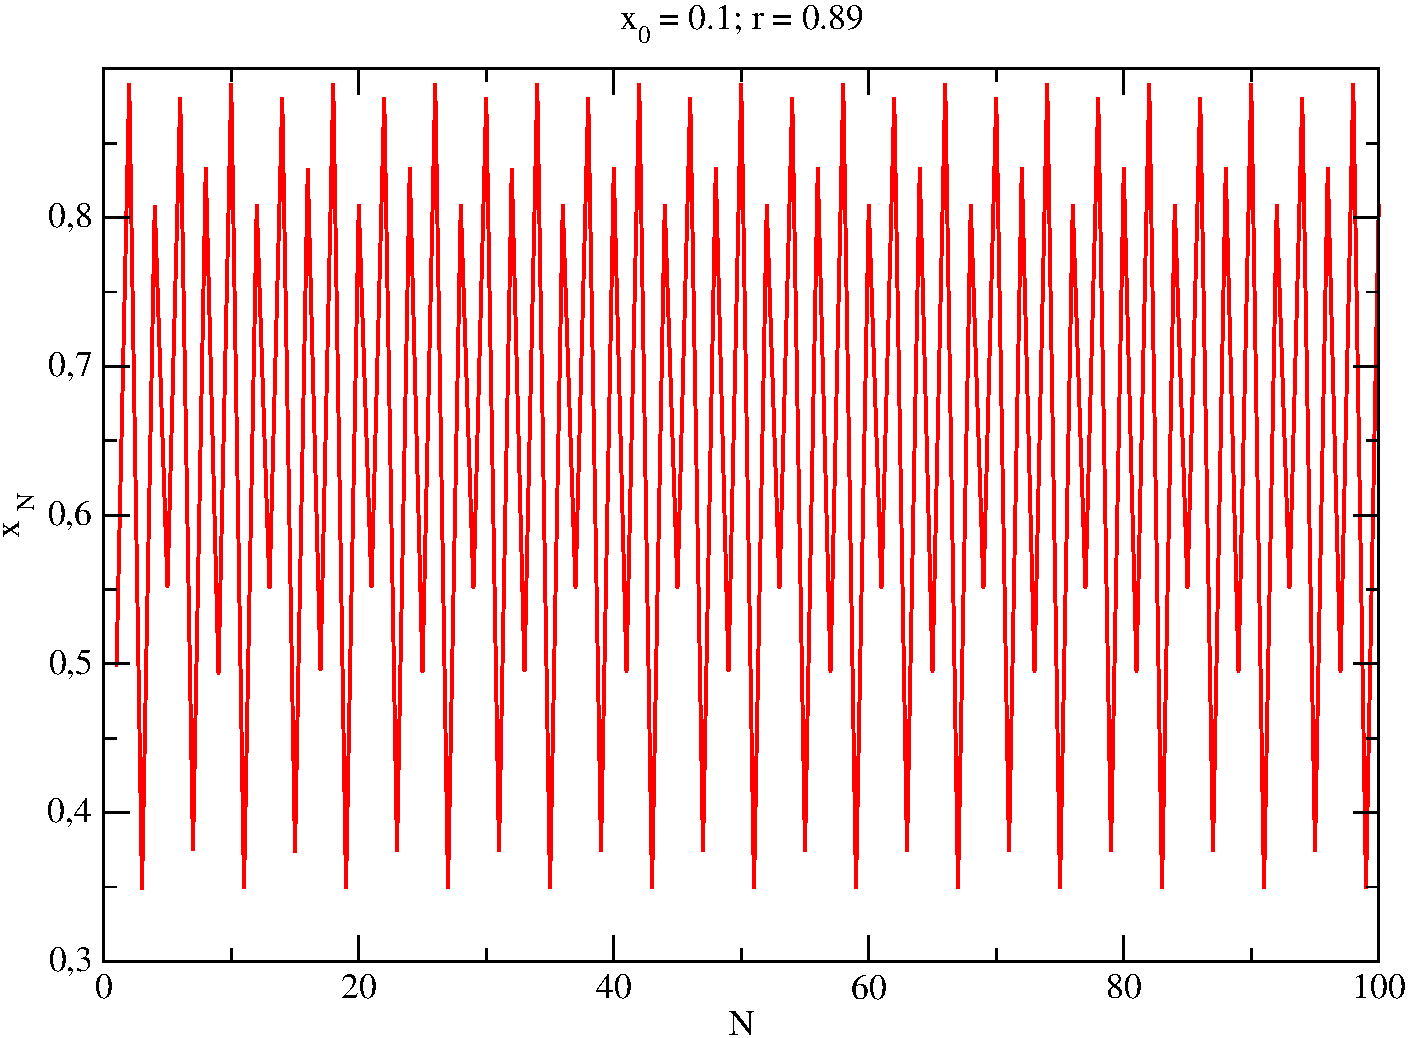
\includegraphics[width=0.447\textwidth]{089.pdf}
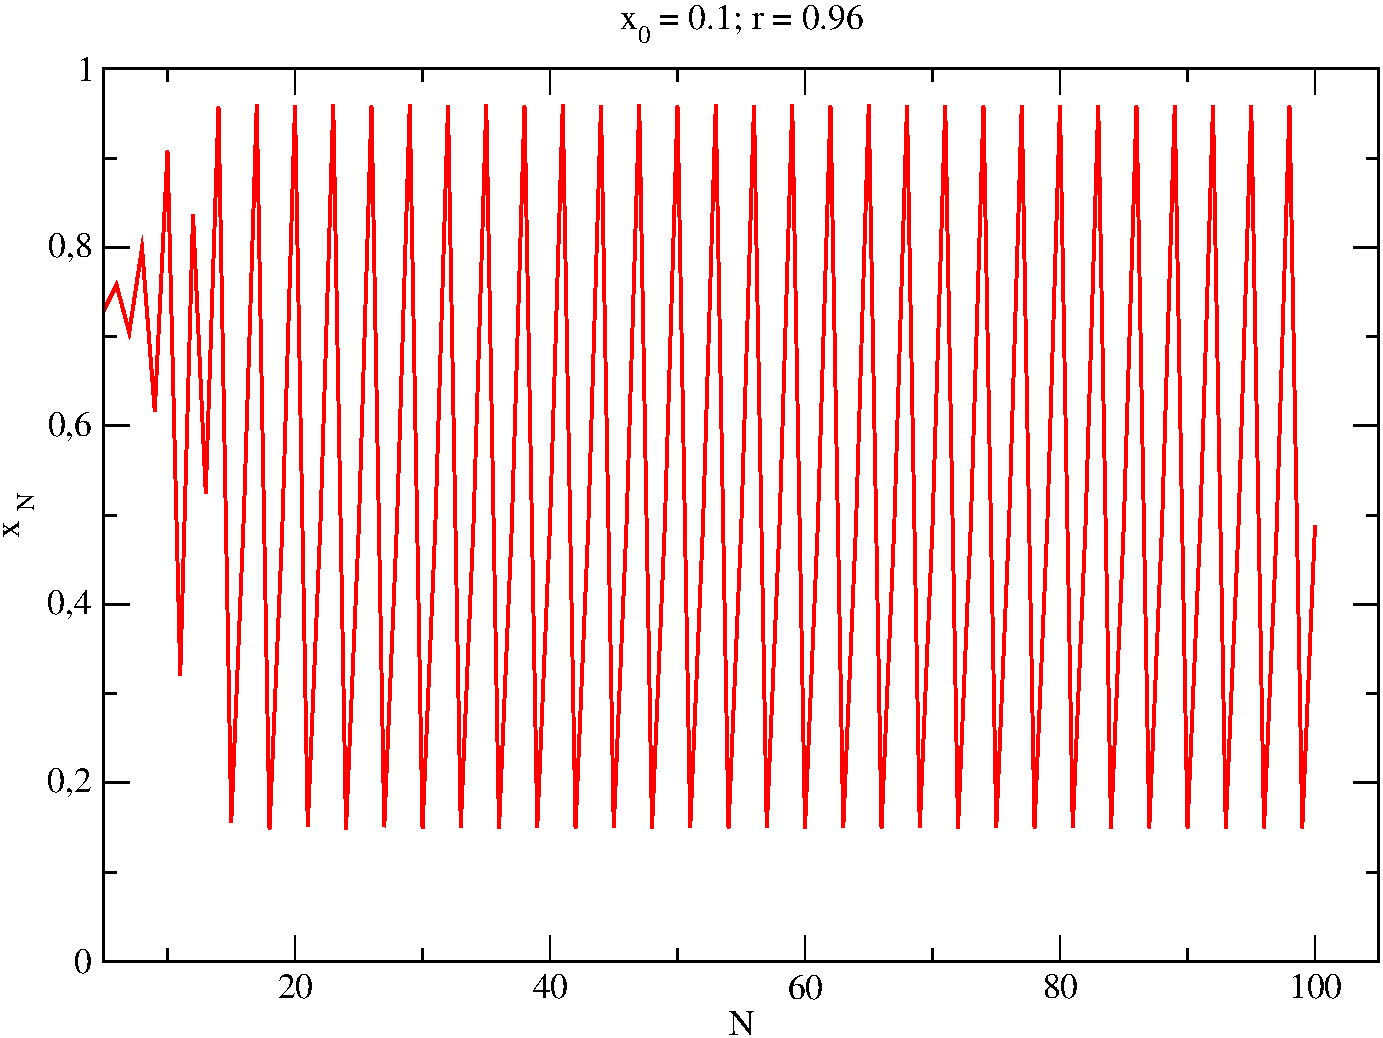
\includegraphics[width=0.447\textwidth]{096.pdf}
\caption{Trajetórias para $x_0 = 0.1$ e r = 0.87(esquerda), r = 0.89 (direita) e r = 0.96 (embaixo). Note que todos apresentam uma solução oscilatória.}
\label{solucao}
\end{figure}


\subsection*{e)}
O valor do expoente de Lyapunov obtido, arrendondado para a segunda casa decimal, foi de $\lambda_{r} = 0.20$. Como  $\lambda_{r} > 0 $ é esperado que as trajetórias sejam caóticas e portanto $\Delta x$ deve crescer expoenencialmente para N pequeno. O resultado pode ser visto na Figura \ref{e)}. É possível perceber que para valores de N até 50 temos que $\Delta x$, em escala logaritmica, cresce (de maneira aproximada) linear com N, como esperado. Porém, para N acima de 75 temos o que parece ser um comportamento oscilatório em torno de $\Delta x = 0.5$.

\begin{figure}[!htb]
\centering
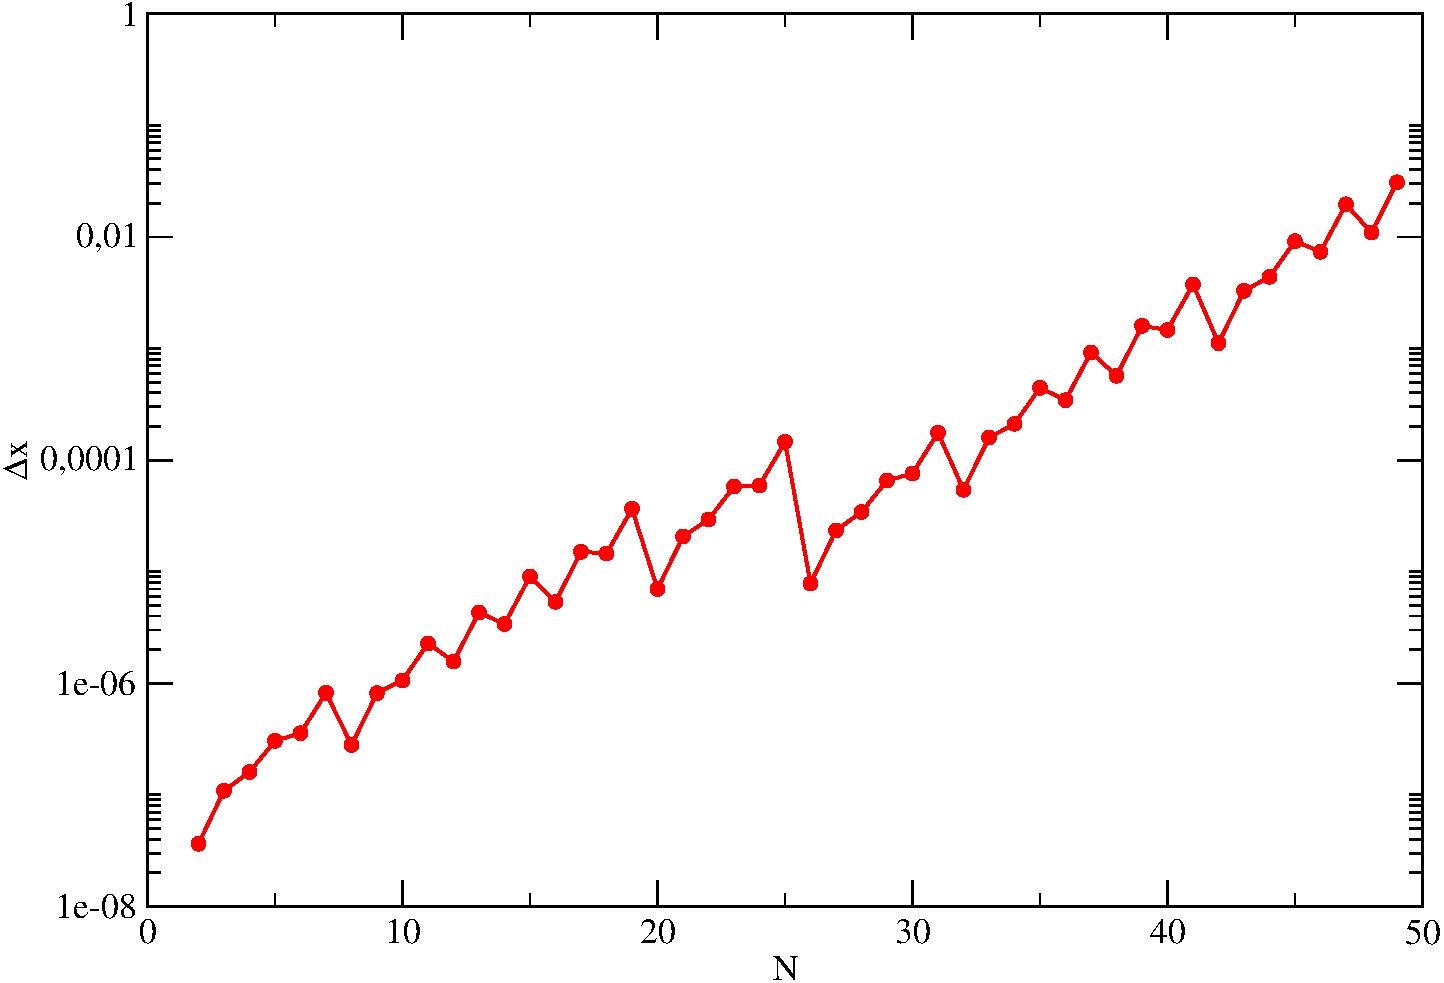
\includegraphics[width=0.447\textwidth]{livro.pdf}
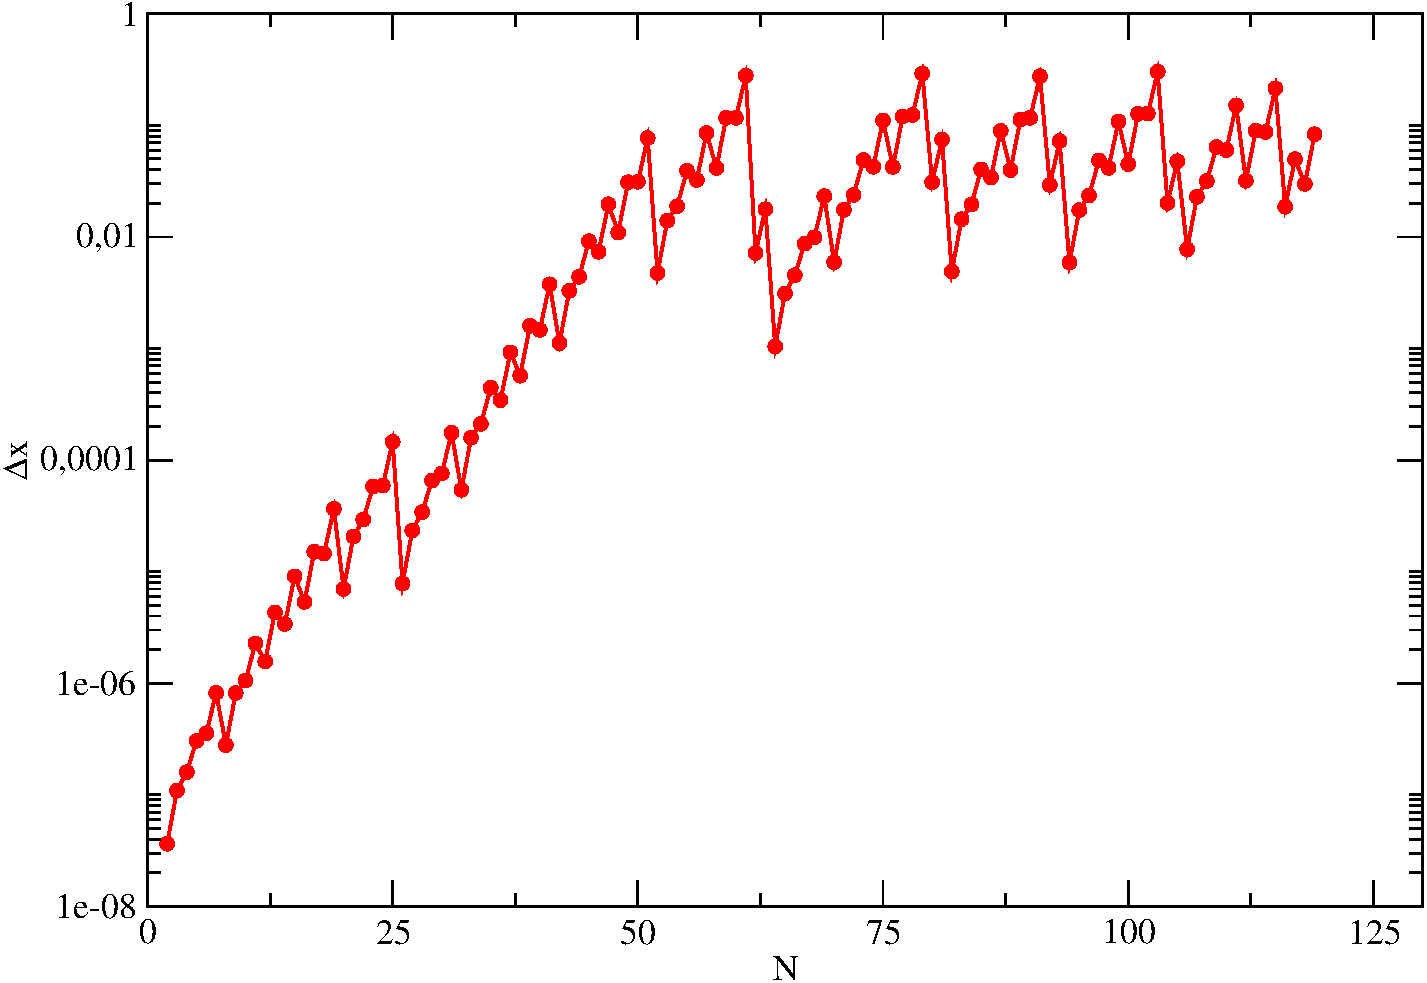
\includegraphics[width=0.447\textwidth]{total.pdf}
\caption{ $\Delta x$ para N até 50 (esquerda) e para N até 125.  }
\label{e)}
\end{figure}


\subsection*{f)}
Os gráficos podem ser vistos na Figura \ref{lambda}. Foi feito um zoom na região $0.7 < r < 1.0$ de modo a ficar claro a comparação com a referência [1]. 
\begin{figure}[!htb]
\centering
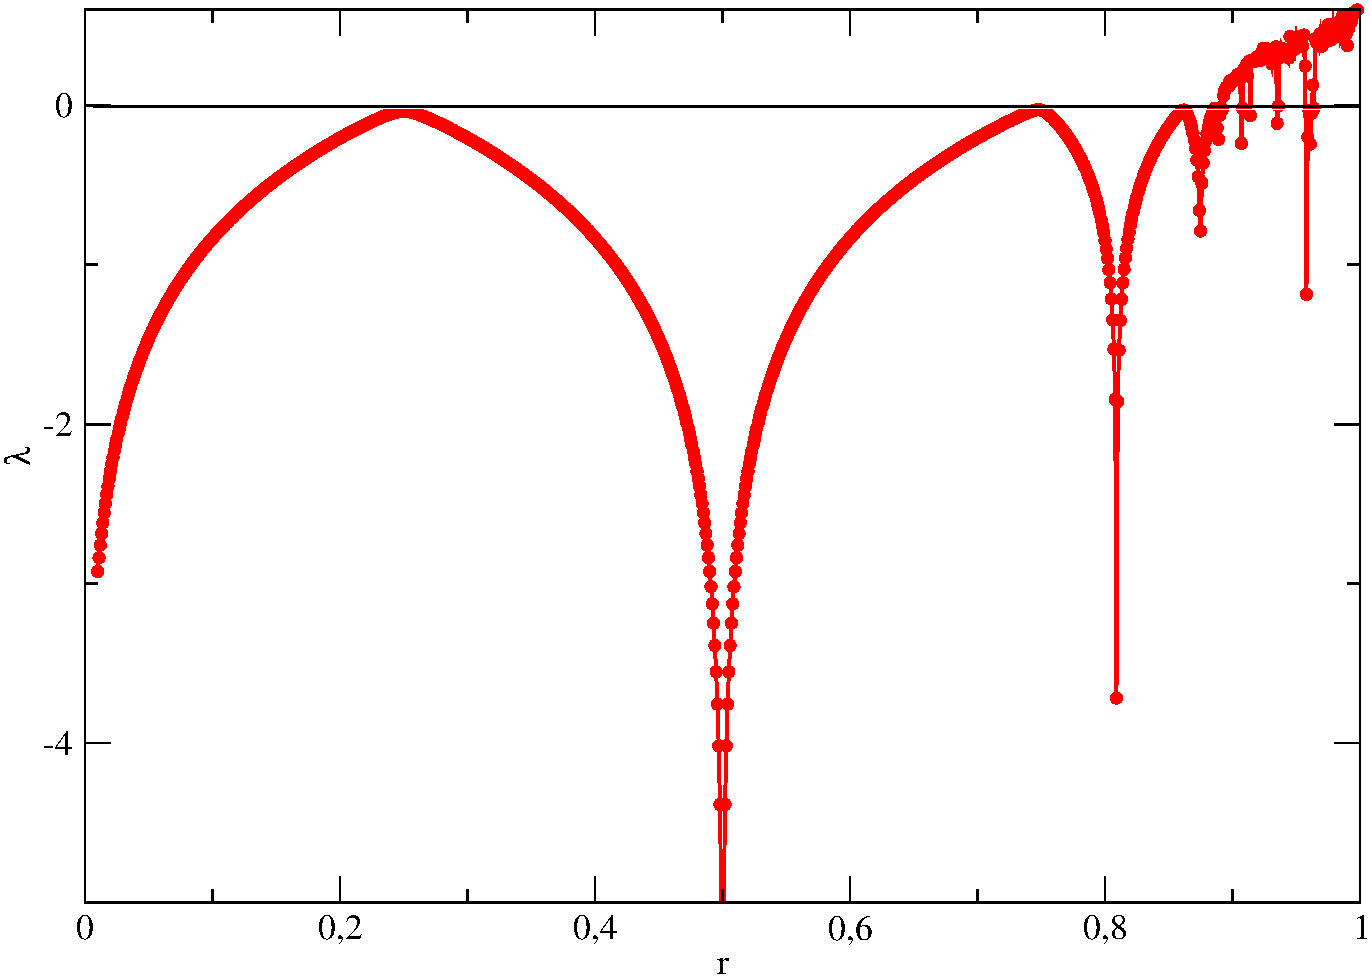
\includegraphics[width=0.447\textwidth]{tudo.pdf}
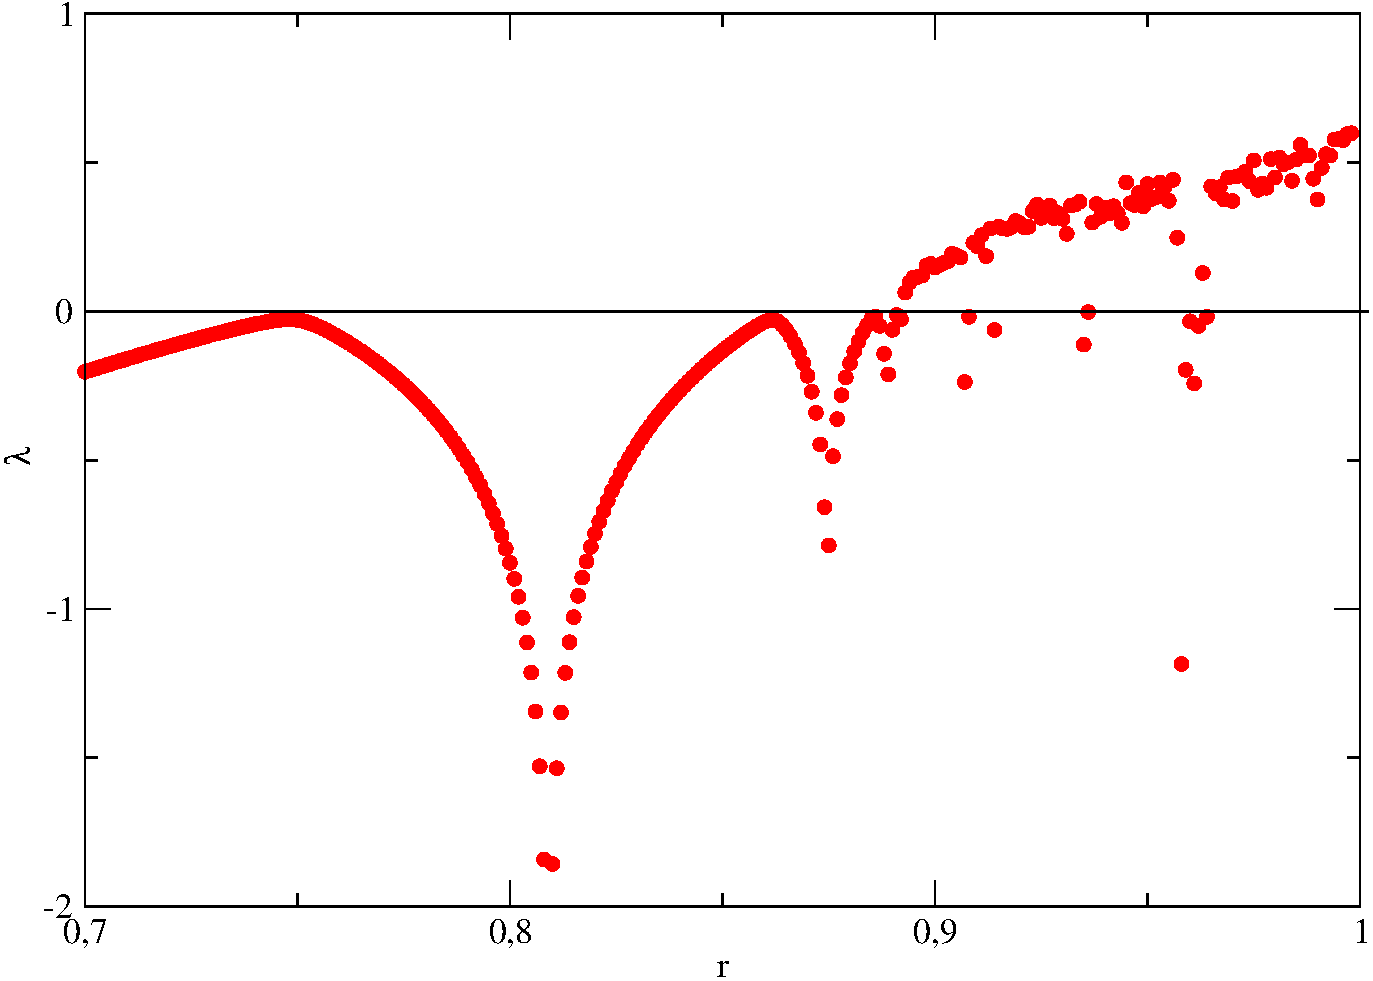
\includegraphics[width=0.447\textwidth]{data.pdf}
\caption{$\lambda$ em função de r com r entre 0 e 1 (esquerda) e o mesmo gráfico com um zoom na região com r entre 0.7 e 1.0 (direita). }
\label{lambda}
\end{figure}

A análise do gráfico mostra que para qualquer valor de $r < 0.85 $ temos um coeficiente $\lambda$ menor do que zero, fato coerente com os itens anteriores onde obtivemos trajetórias estáveis para todo $ r < 0.73$ e trajetórias instáveis para $r > 0.85$. O único ponto onde poderíamos ter problema é em r = 0.25, que possui um coeficiente $\lambda = 0$. Mas já sabíamos disto da análise de estabilidade feita no item a), pois r = 0.25 faz com que os dois valores de $x^*$ sejam marginais.

\subsection*{g)}

Baseado na figura \ref{lambda} foi feito um programa pra calcular qual valor de r faz com que $\lambda$ seja o mais próximo de zero em quatro regiões distintas: em torno de 0.75, em torno de 0.85 e pra dois valores entre 0.85 e 0.90. Os valores encontrados estão apresentados na tabela 1. Os valores de r foram aproximados para a terceira casa decimal e o valor de lambda associado foi arredondado para a primeira casa decimal. Caso um valor mais preciso seja necessario basta verificar a saída de dados do programa na tela.

\begin{table}[!h]
\centering
\begin{tabular}{|l|l|l|l|l|}
\hline
r  & $\lambda$   \\ \hline
0.743  & 2$\times 10^{-3}$  \\ \hline
0.864 & 9$\times 10^{-5}$   \\ \hline
0.886 & 1$\times 10^{-5}$  \\ \hline
0.897 & 4$\times 10^{-5}$  \\ \hline
\end{tabular}
\caption{Valores de r e $\lambda$ encontrados}
\label{tabela1}
\end{table}

A comparação com a referência [1] mostra desvios a partir da terceira casa decimal, o que pode ser explicado ao se considerar que usamos um dr = 0.001. Além disso, a referência traz 5 outros valores de r entre 0.891 e 0.893, que nosso programa é incapaz de calcular com um dr tão grande. Foi feito um outro programa (tentativa2.f90) para corrigir este problema, mas não foram obtidos resultados satisfatórios devido a dificuldade de juntar a precisão necessária com a habilidade de excluir soluções inadequadas (como soluções próximas da solução correta exata, que ainda estão na margem de erro).


\section*{Exercício 2}

\subsection*{a)}
Dada a relação $f^{1}_{r}(\omega_i) = \omega_{i+1} = (1-r)\omega_i$ temos que o ponto fixo é dado por:

\begin{equation}
\omega^* = (1-r)\omega^* = 0
\end{equation}

Este ponto fixo é estável desde que:

\begin{equation*}
|f'^1_r(\omega_i) | < 1
\end{equation*}
\begin{equation*}
-1 < (r-1) < 1   
\end{equation*}
\begin{equation}
0 < h < 2\tau   
\end{equation}

Na Figura \ref{taubom} temos o resultado do cálculo da derivada com $h \ll \tau$. Foi escolhido $h =\tau \times 10^{-5} $. A solução exata e a solução numérica estão tão próximas que é impossível distingui-las uma da outra. Portanto foi escolhido plotar alguns pontos particulares da solução numérica, de modo a ficar claro o quão bem a curva exata se ajusta aos pontos.

\begin{figure}[!htb]
\centering
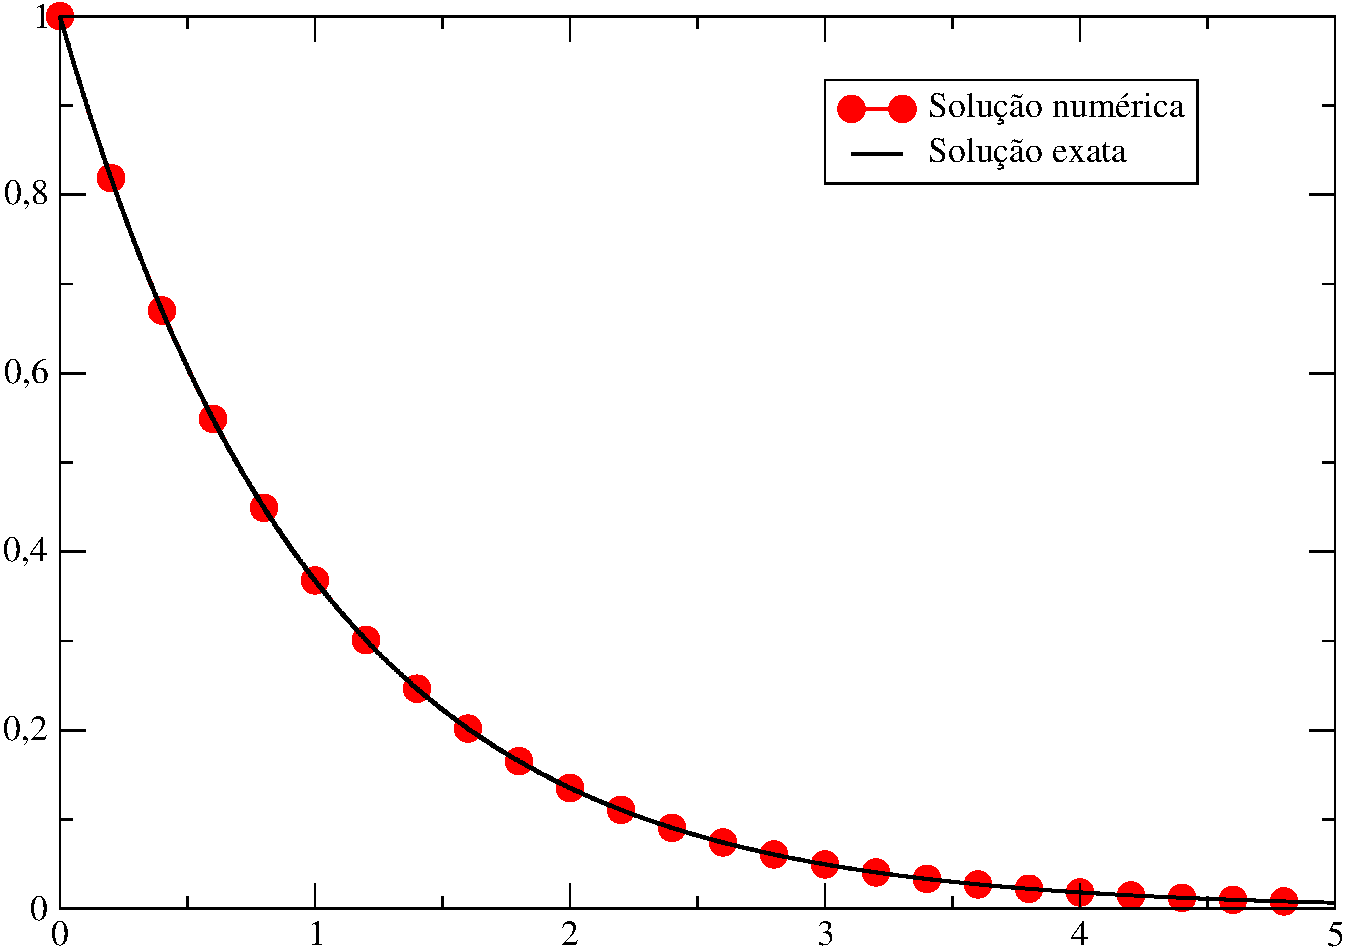
\includegraphics[width=0.447\textwidth]{taubom.pdf}
\caption{ Derivada com $h = 0.00001 \tau $.  }
\label{taubom}
\end{figure}

Na Figura \ref{tau} temos os gráficos da derivada para vários valores de $h = h_{max} \pm \epsilon$, com $\epsilon = 0.1$. Podemos ver no gráfico da esquerda que para $h = h_{max} + \epsilon$ a curva obtida diverge da curva exata com cada termo que é adicionado, ao passo que a curva da direita, apesar de não ser uma boa aproximação, tende a convergir para a curva exata com cada N.


\begin{figure}[!htb]
\centering
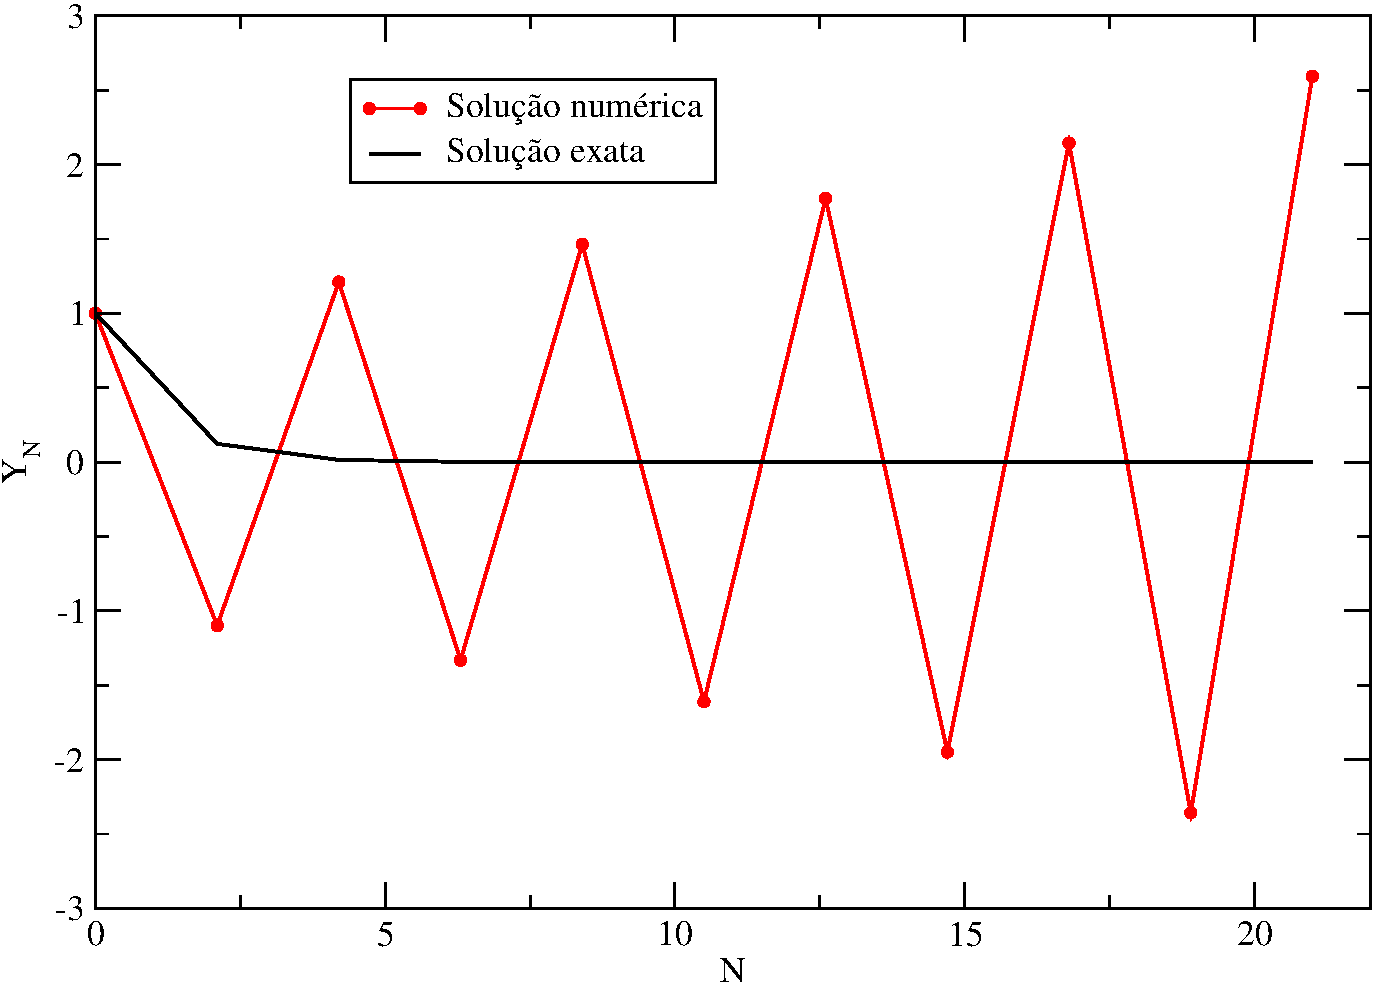
\includegraphics[width=0.447\textwidth]{1-1.pdf}
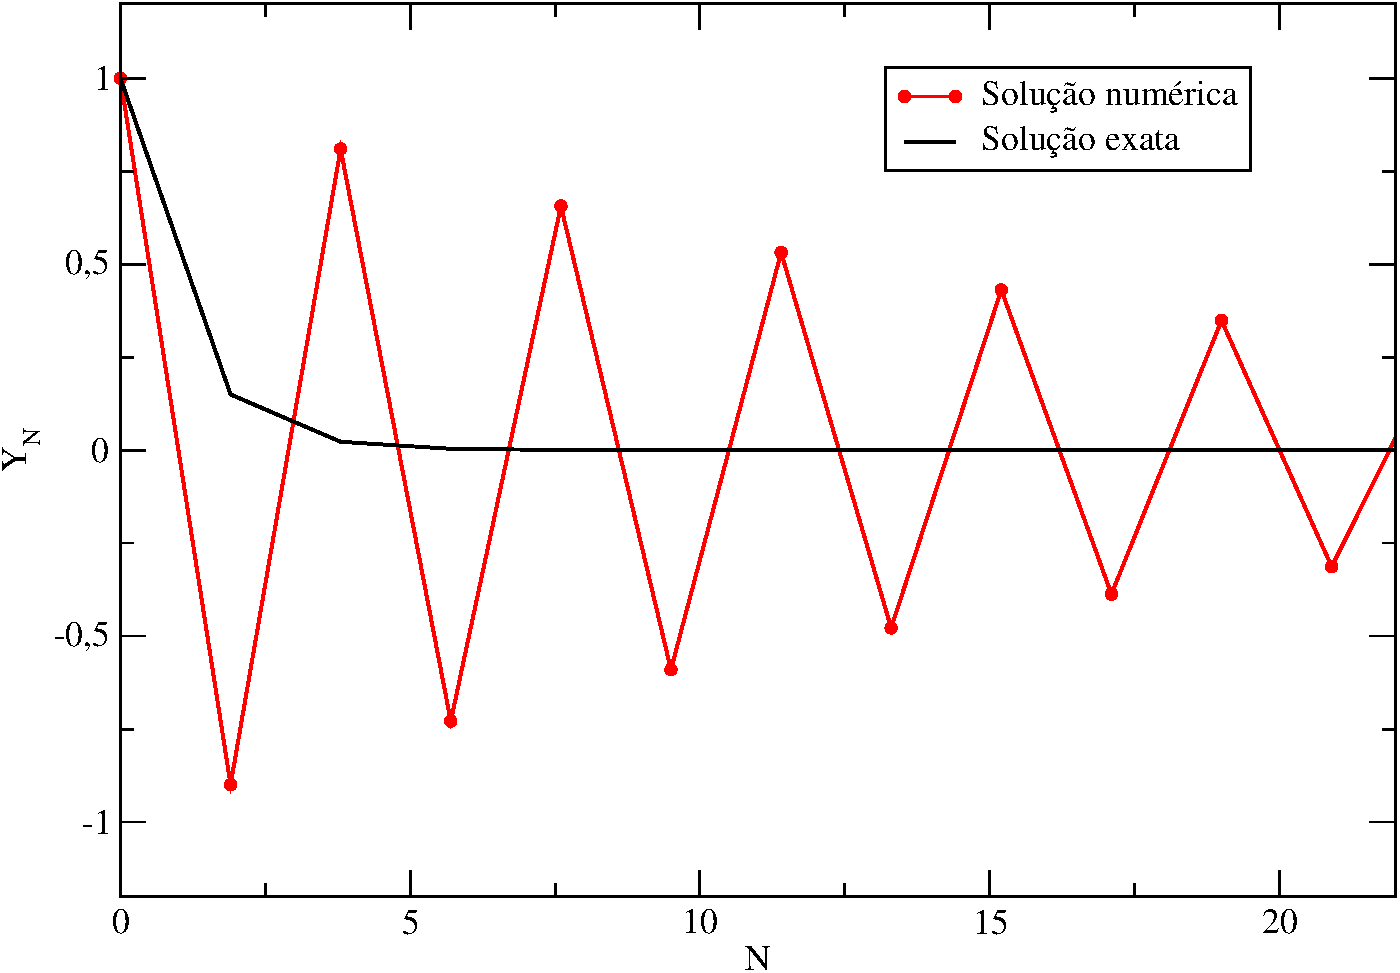
\includegraphics[width=0.447\textwidth]{1-2.pdf}
\caption{ Derivada, com $\epsilon = 0.1$, para valores $ h = h_{max} + \epsilon $ (esquerda) e para valores $ h = h_{max} - \epsilon $ (direita)  }
\label{tau}
\end{figure}

Na Figura \ref{tau2} foi feito o mesmo cálculo para um $\epsilon = 0.5$, o que torna a diferença entre as duas curvas mais evidente. No gráfico da esquerda é possivel observar pelos valores do eixo y como a curva numérica se afasta da curva exata. Já no gráfico da direita vemos que a partir de N = 10 temos que a curva numérica já se apresenta como aproximação razoável para a curva exata.


\begin{figure}[!htb]
\centering
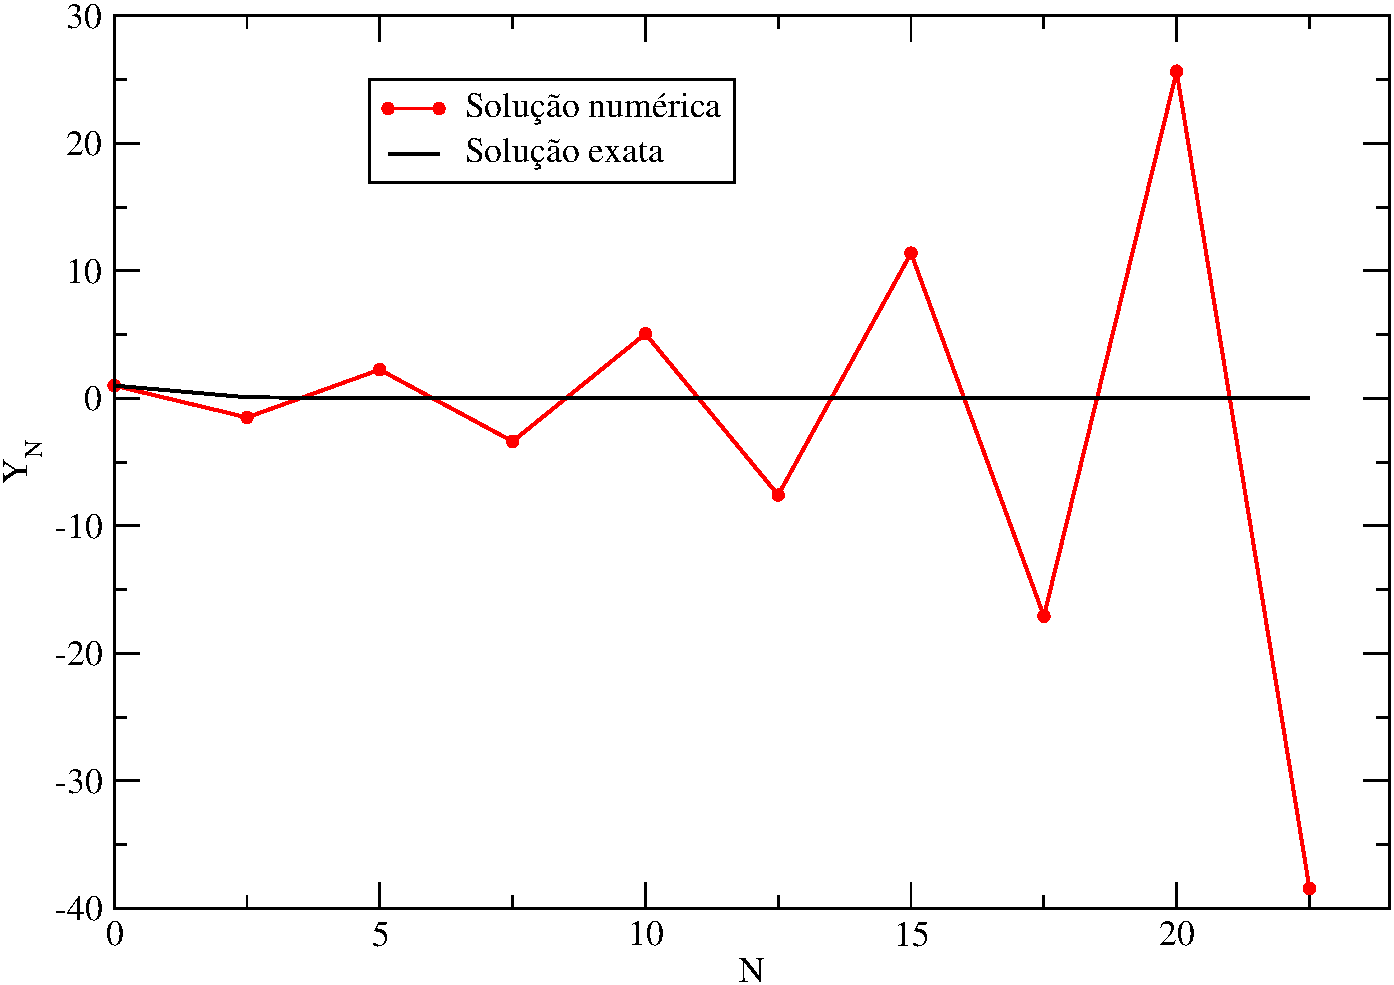
\includegraphics[width=0.447\textwidth]{2-1.pdf}
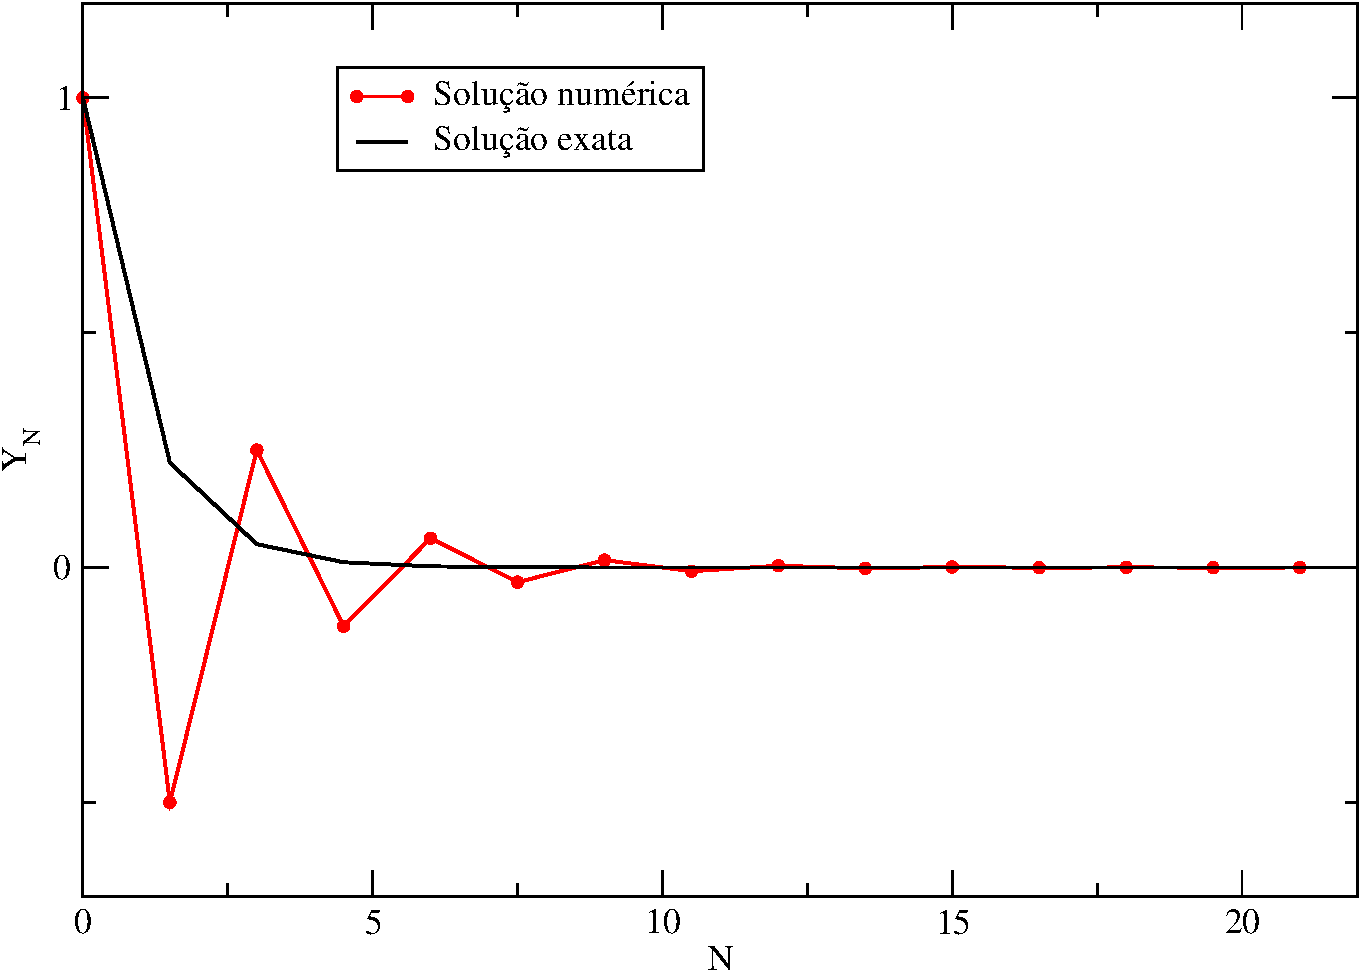
\includegraphics[width=0.447\textwidth]{2-2.pdf}
\caption{ Derivada, com $\epsilon = 0.5$, para valores $ h = h_{max} + \epsilon $ (esquerda) e para valores $ h = h_{max} - \epsilon $ (direita)  }
\label{tau2}
\end{figure}



Neste caso a matriz de amplificação $\textbf{G}$ é uma matriz 1x1 dada por: 

\begin{equation}
\textbf{G} = \frac{\partial T(x)}{\partial x} = (1-r)
\end{equation}

Cujo autovalor $\lambda$ é dado pela equação:

\begin{equation}
 (1-r) - \lambda = 0   \Rightarrow \lambda = (1-r)
\end{equation}

A exigência de que $|\lambda| < 1$ imediatamente reproduz a Eq. (5).

\subsection*{b)}

Temos que 

$\begin{cases} 
\dot{x} = ax + by \\ 
\dot{y} = cx + dy
\end{cases} $

Utilizando o método de Euler podemos escrever esta equação da seguinte forma:

\begin{equation}
\begin{cases} 
$$w^x_{i+1} = f^x(w^x_i,w^y_i) = (ah + 1)w^x_i +(hb)w^y_i \\ 
w^y_{i+1} = f^y(w^x_i,w^y_i) = (dh + 1)w^y_i +(hc)w^x_i $
$\end{cases}
\end{equation}

O que nos dá uma matriz $\textbf{G}$ da forma:

\[
\textbf{G}
=
\begin{bmatrix}
    ah + 1 & hc \\
    hb & dh + 1 
\end{bmatrix}
\]

Cujos autovalores são dados pela equação:

\begin{equation}
(1 + ah - \lambda)(hd + 1 -\lambda) - h^2bc = 0
\end{equation}

Fazendo a = 1; b = 1; c = 4 e d = -2 ficamos com:

\begin{equation}
\lambda^2 + (h-2)\lambda + ( -6h^2 -h + 1) = 0
\end{equation}

cujo discriminante é:

\begin{equation*}
\Delta = (h^2 -4h + 4 + 24h^2 + 4h -4) = 25h^2
\end{equation*}

E portanto as soluções são:

\begin{equation}
\begin{cases} 
$$\lambda_1 = (1+2h) \\ 
\lambda_2   = (1-3h)  $
$\end{cases}
\end{equation}

A estabilidade é dada por:

\begin{equation}
\begin{cases} 
-1 < (1+2h) < 1 \\ 
-1 < (1-3h) < 1  $
$\end{cases}
\end{equation}

\begin{equation}
\begin{cases} 
-1 < h < 0 \\ 
 0 <  h < 2/3  $
$\end{cases}
\end{equation}

Ou seja, não existe valor de h que satisfaça as duas equações ao mesmo tempo. Para resolver numericamente foi escolhido h = 0.2, na faixa que permite solução estável para uma das equações, e h = -0.2, que permite solução estável para a outra equação. A solução para h = 0.2 está na Figura \ref{2}.


\begin{figure}[!htb]
\centering
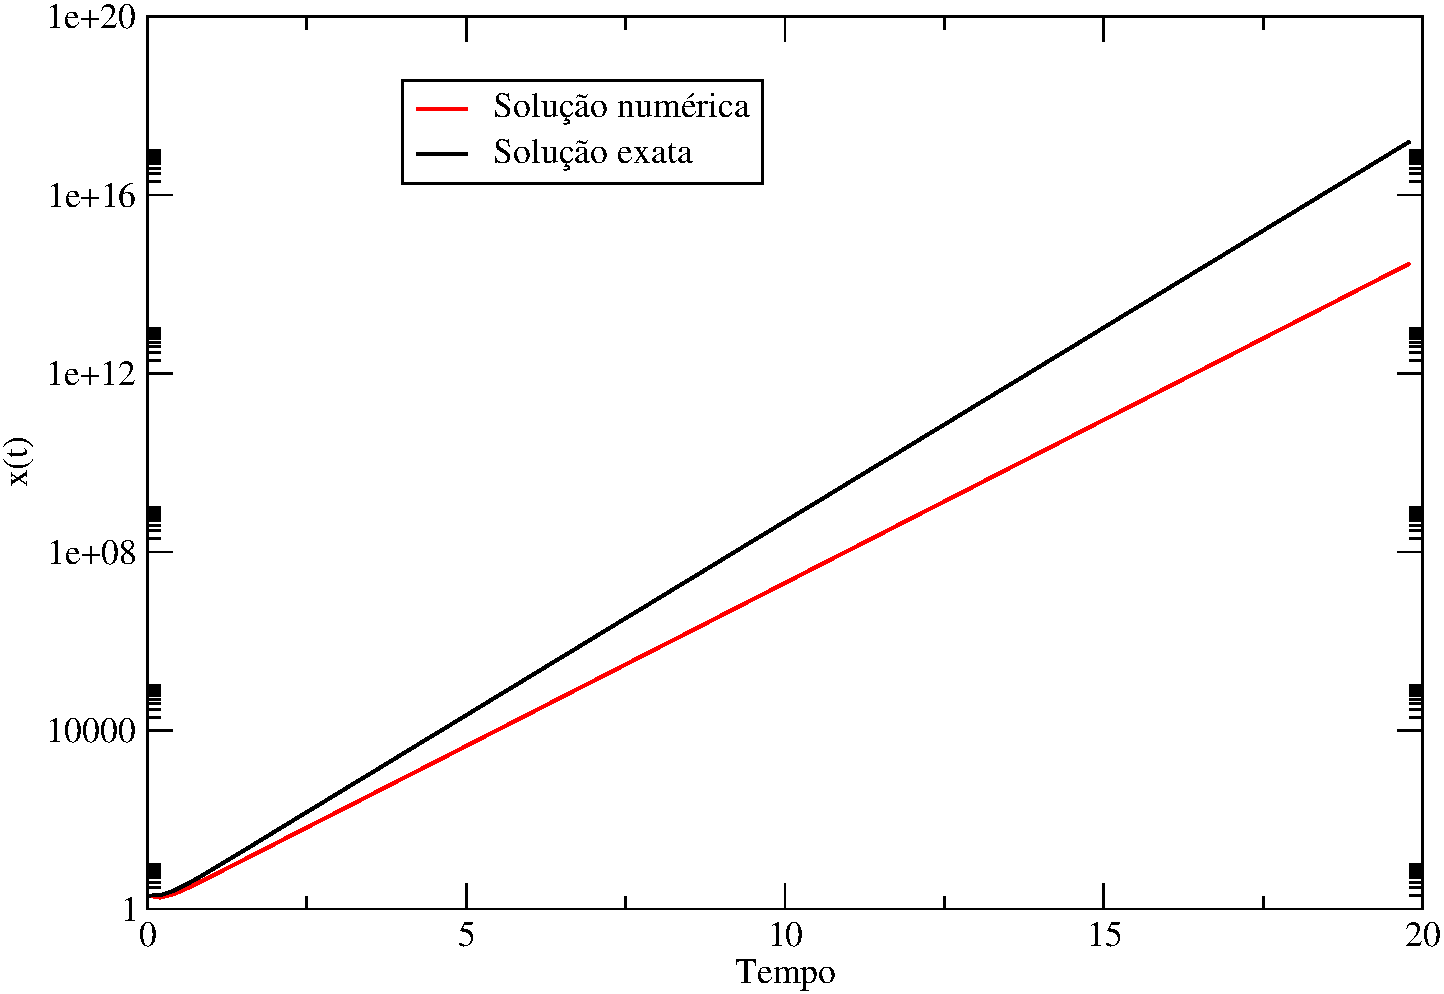
\includegraphics[width=0.447\textwidth]{x.pdf}
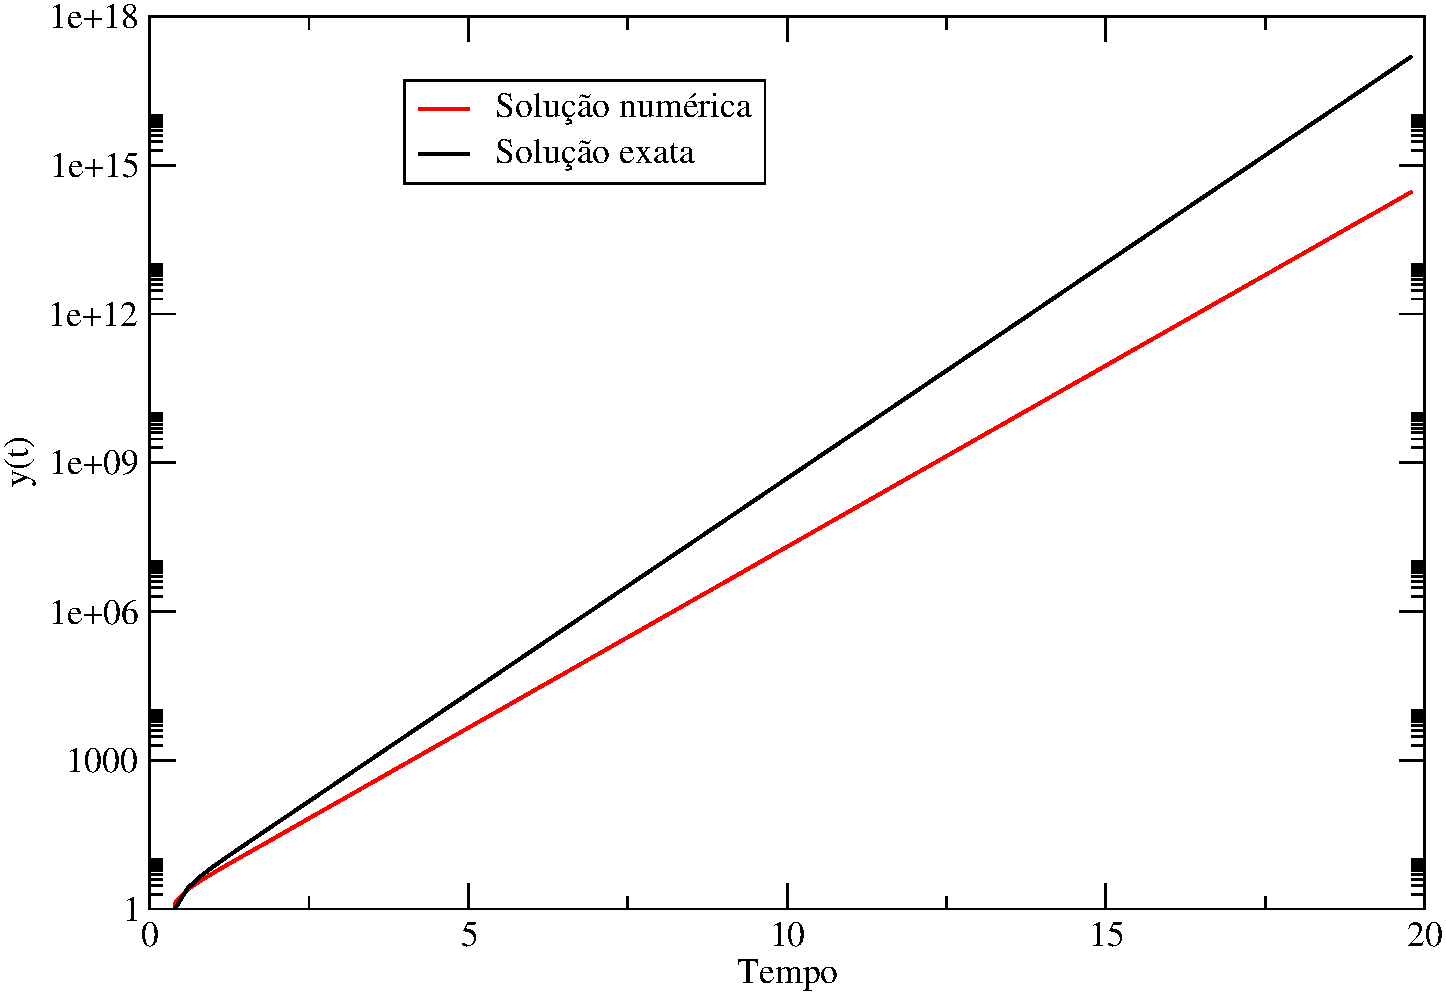
\includegraphics[width=0.447\textwidth]{y.pdf}
\caption{ Solução da EDO acoplada para x (esquerda) e y (direita) com h = 0.2.  }
\label{2}
\end{figure}

Como pode ser visto tanto a solução para x(t) quanto para y(t) divergem da solução exata com o passar do tempo. Alguém poderia argumentar que uma das soluções deveria convergir, visto que o parâmetro h é estável para ela, mas o fato das equações serem acopladas faz com que caso uma divirja a outra também deve divergir.

Na Figura \ref{22} temos a mesma solução para o caso h = -0.2. Inverter o sinal de h fez com que a solução para y(t) invertesse o sinal e ficasse negativa, o que impossibilitou o gráfico ser feito em escala logaritmica. 

\begin{figure}[!htb]
\centering
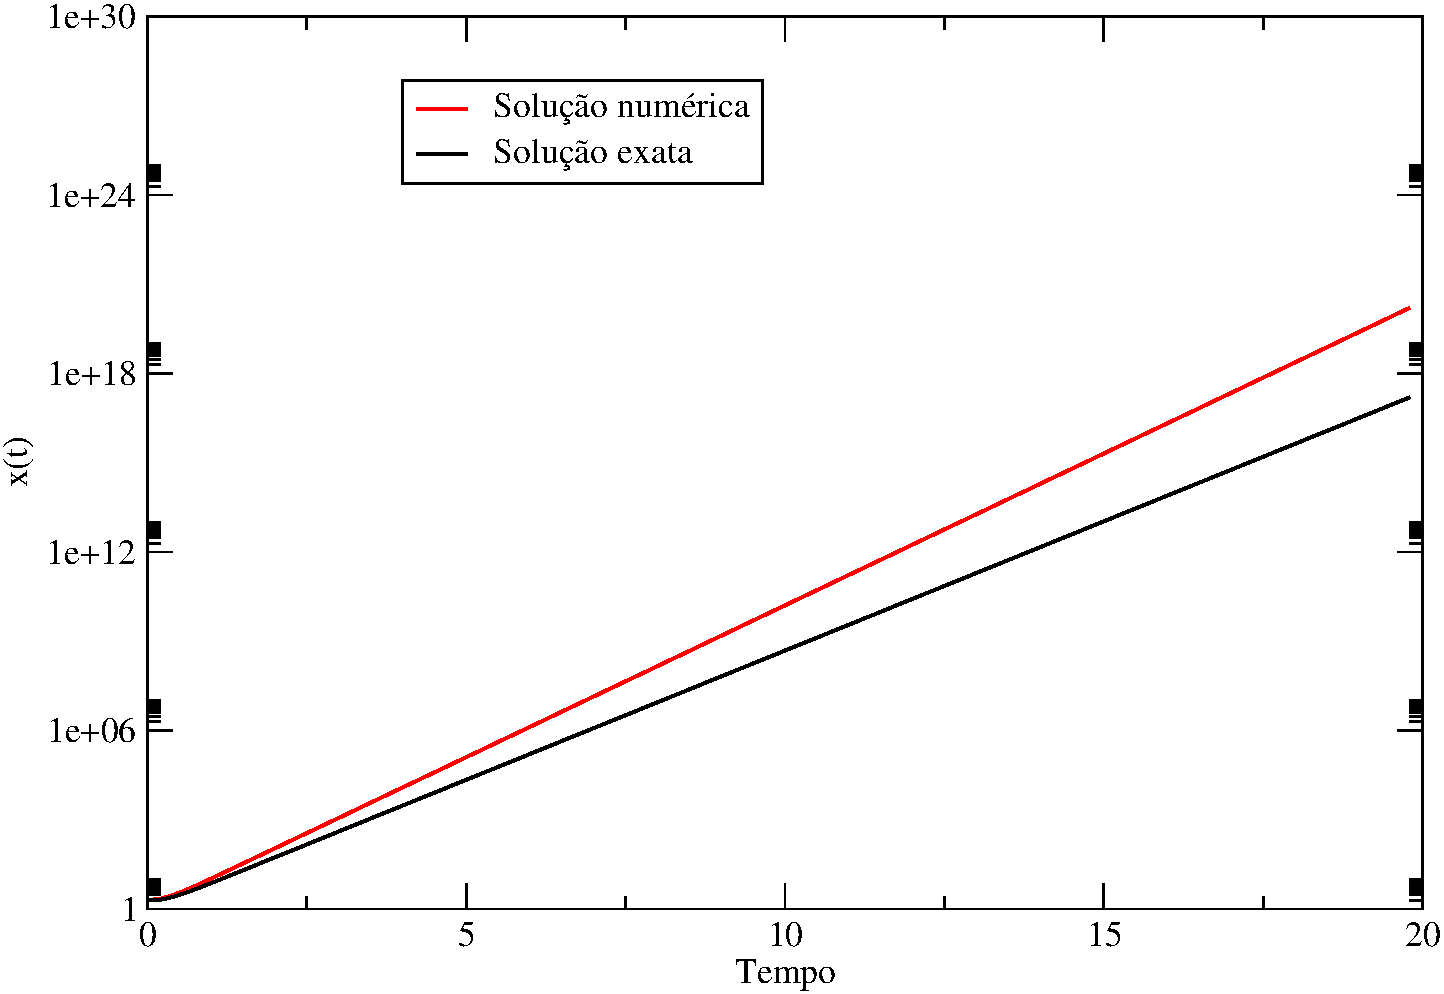
\includegraphics[width=0.447\textwidth]{x2.pdf}
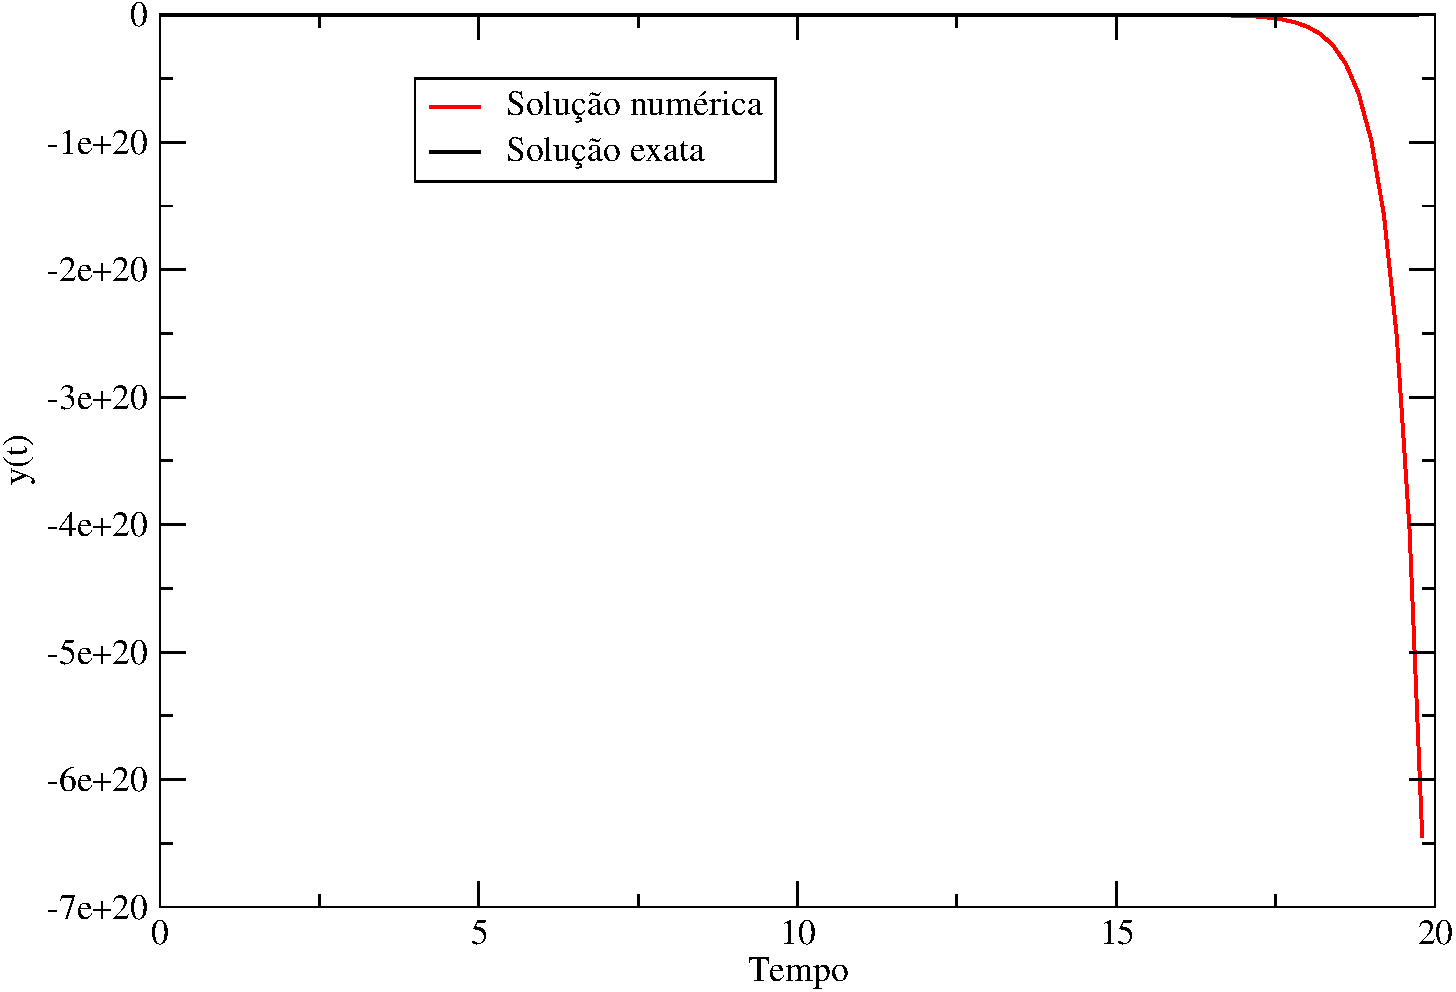
\includegraphics[width=0.447\textwidth]{y2.pdf}
\caption{ Solução da EDO acoplada para x (esquerda) e y (direita) com h = -0.2. A solução exata para y(t) é indistinguivel da reta y = 0 nesta escala.  }
\label{22}
\end{figure}

\section*{Exercício 3}
\subsection*{a)}
Na Figura \ref{p1} podemos ver o espaço de fase do oscilador harmônico para o conjunto de parâmetros pedidos.

\begin{figure}[!htb]
\centering
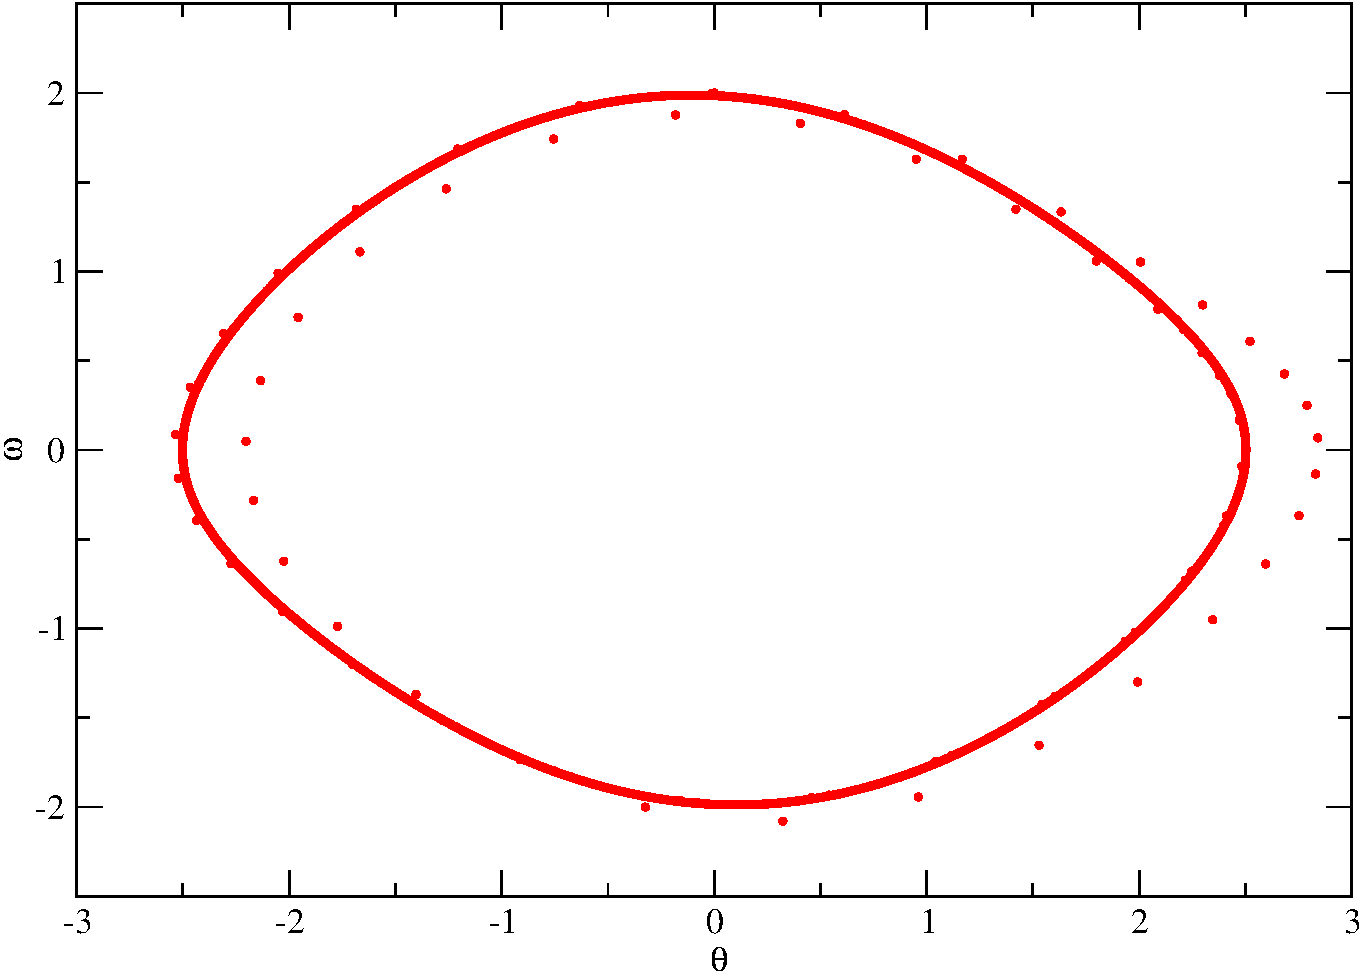
\includegraphics[width=0.447\textwidth]{p1.pdf}
\caption{Espaço de fase para o oscilador harmônico com b = 0.9.  }
\label{p1}
\end{figure}



\vspace{3pt}
\subsection*{b)}
Na Figura \ref{p2} temos o espaço de fase para o outro conjunto de parâmetros. Trata-se de uma órbita que não é fechada, típica de sistemas caoticos. Ainda é possível ver a curva da Figura \ref{p1} quase como uma envoltória. Note que este gráfico aparenta ter sido cortado em $x = \pm3$, mas isto se deve ao fato de que pela dinâmica do problema temos que $\theta$ está confinado no intervalo $\left[ -\pi,\pi\right]$. No caso anterior a partícula não era capaz de ter uma amplitude maior que $\pi$, mas neste caso temos uma força externa maior e isto já é possível.

\begin{figure}[!htb]
\centering
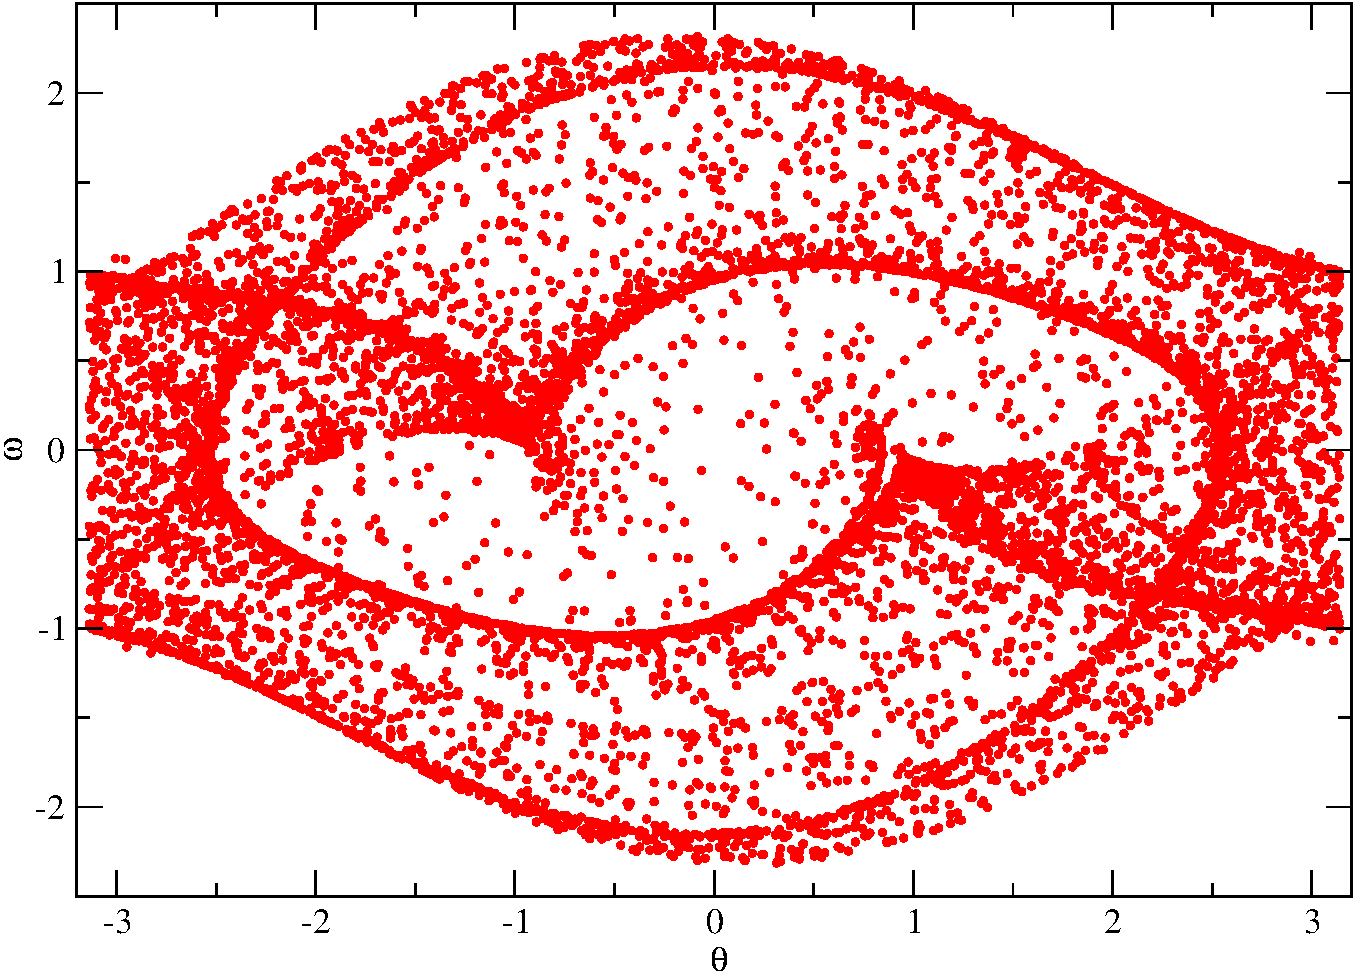
\includegraphics[width=0.447\textwidth]{p2.pdf}
\caption{ Espaço de fase para o oscilador com b = 1.15.  }
\label{p2}
\end{figure}



\subsection*{c)}

Na Figura \ref{a12} temos o espaço de fase das duas situações anteriores plotados em conjunto com uma situação que possui configuração inicial próxima. Foi escolhido mudar a velocidade inicial de $\omega = 2.00$ para $\omega = 1.98$ e a posição inicial de $x_0 = 0$ para $x_0 = 0.01$. Os gráficos, em especial do sistema não-caótico, são extremamente parecidos entre si, de modo que foi necessário omitir alguns pontos vermelhos para que os pontos pretos pudessem ser vistos; por isto que o gráfico da esquerda não apresenta uma linha vermelha contínua. Estes gráficos mostram que um deslocamento infinitesimal geram pequenas mudanças no espaço de fase.

\begin{figure}[!htb]
\centering
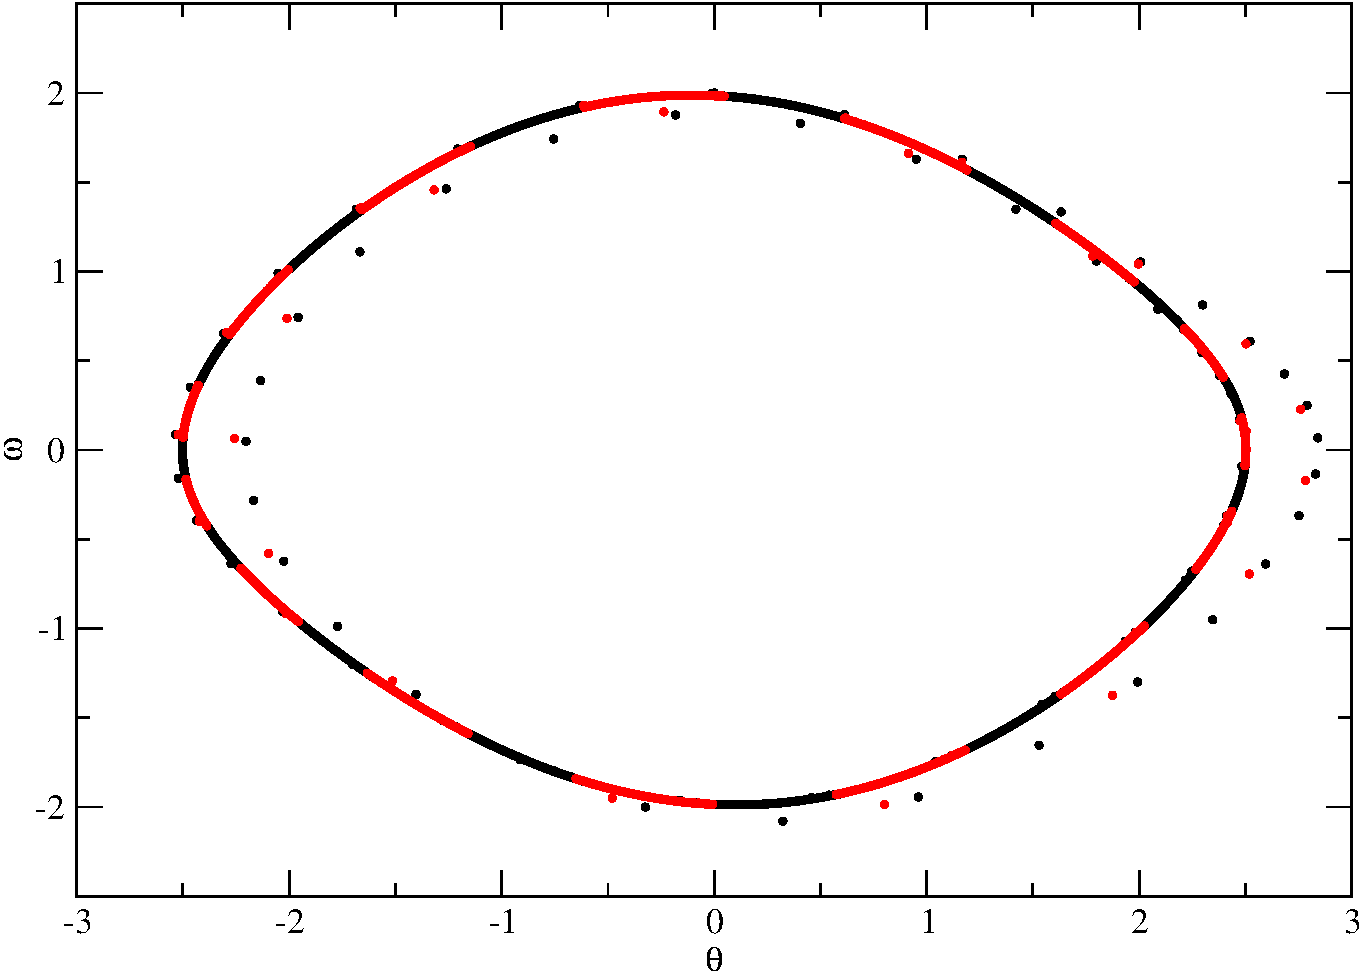
\includegraphics[width=0.447\textwidth]{1ab.pdf}
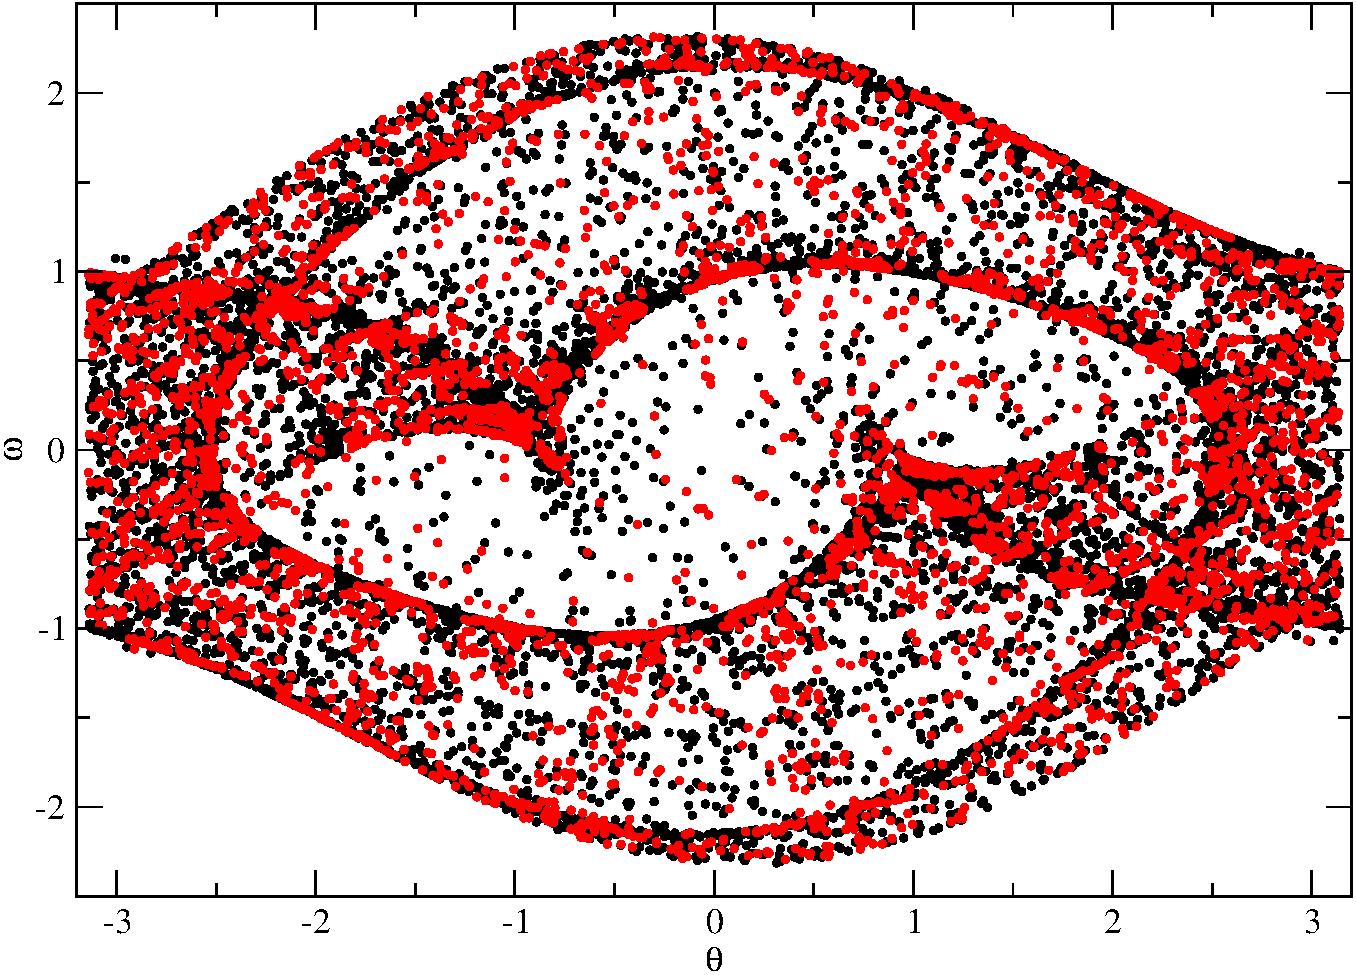
\includegraphics[width=0.447\textwidth]{2ab.pdf}
\caption{ Espaço de fase para duas configurações iniciais próximas para b = 0.9 (esquerda) e b = 1.15 (direita). Alguns pontos vermelhos foram omitidos de modo a melhorar a visualização dos pontos pretos.  }
\label{a12}
\end{figure}


\end{document}
